\documentclass[11pt,a4paper,twoside,asymmetric]{article}
\usepackage[english]{babel}
\usepackage{amsmath}
\usepackage{amsfonts}
\usepackage{amssymb}
\usepackage{graphicx}
\usepackage[left=3cm,right=2.5cm,top=3.5cm,bottom=2.5cm,%
headsep=0.75cm,headheight=2cm,footskip=1cm]{geometry}
\usepackage[dvipsnames]{xcolor}
\usepackage{fancyhdr}
\usepackage{tabularx}
\usepackage{booktabs}
\usepackage{float}
\usepackage{placeins}
\usepackage{titlesec}
\usepackage[labelsep=period]{caption}
\usepackage{multirow}
\usepackage{indentfirst}
\usepackage{xpatch}
\usepackage{setspace}
\usepackage{newtxtext}
\usepackage[labelfont=bf,font=small]{caption}
\captionsetup[table]{skip=6pt}

\usepackage{hyperref}
\hypersetup{
    colorlinks=true,
    linkcolor=RoyalBlue,
    urlcolor=RoyalBlue,
    citecolor=RoyalBlue,
    citebordercolor=0 0 1
    }
\urlstyle{same}

\addto\captionsenglish{\renewcommand{\figurename}{\textbf{\small{Fig.}}}}
\addto\captionsenglish{\renewcommand{\tablename}{\textbf{\small{Table}}}}

\titlespacing{\section}{0pt}{12pt}{4pt}
\titleformat{\section}[hang]{\large\bfseries}{\thesection. }{0.0em}{}

\titlespacing{\subsection}{0pt}{6pt}{3pt}
\titleformat{\subsection}[hang]{\bfseries}{\thesubsection. }{0.0em}{}

\renewcommand{\headrulewidth}{1.5pt}
\xpretocmd\headrule{\color{RoyalBlue}}{}{\PatchFailed}

\renewcommand{\footrulewidth}{1.5pt}
\renewcommand{\footrule}{\hbox to\headwidth{%
  \color{RoyalBlue}\leaders\hrule height \headrulewidth\hfill}}

\setlength{\parskip}{0.3em}
\raggedbottom
\widowpenalty=10000
\clubpenalty=10000

% BẢN TIẾNG VIỆT NỘI BỘ -- không nộp. Đây là bản gốc để hiệu đính trước khi dịch
% sang paper/ijrcs/IJRCS_CCKD_SSVEP.tex (bản tiếng Anh), theo quy tắc ghi trong
% bo-nao-claude/memory.md (2026-11-01): viết tiếng Việt trước, hiệu đính, rồi mới dịch.
% BUILD: dịch bằng xelatex (không phải pdflatex) -- newtxtext dưới pdflatex (mã hoá
% OT1/8-bit) không có dấu tiếng Việt; xelatex dùng bản OpenType TeXGyreTermesX nên
% hiển thị Unicode đầy đủ. Lệnh: xelatex IJRCS_CCKD_SSVEP_vi.tex (chạy 2 lần).
\newcommand{\tbd}[1]{\textcolor{red}{[CHƯA CÓ: #1]}}
\newcommand{\chuaduyet}[1]{\textcolor{OliveGreen}{[CẦN TÁC GIẢ DUYỆT: #1]}}

\fancypagestyle{firstpage}{
\fancyhf{}
\lhead{
\includegraphics[scale=0.15]{ijrcs}\\}
\rhead{
\includegraphics[scale=0.09]{ascee}\\}
\chead{International Journal of Robotics and Control Systems\\
\small{Vol. X, No. X, 2026, pp. X-X\\
ISSN 2775-2658\\
\url{http://pubs2.ascee.org/index.php/ijrcs}}}
\rfoot{
\includegraphics[scale=0.3]{email} \small{\href{mailto:ijrcs@ascee.org}{ijrcs@ascee.org}}}
\lfoot{
\includegraphics[scale=1]{doi} \small{\url{http://dx.doi.org/10.31763/ijrcs.v1i1.}}}
}

\fancypagestyle{followingpage}{
\fancyhf{}
\fancyhead[RE,LO]{\small{ISSN 2775-2658\\}}
\fancyhead[LE,RO]{\small{\textbf{\thepage}\\}}
\fancyhead[CE,CO]{International Journal of Robotics and Control Systems\\
\small{Vol. X, No. X, 2026, pp. X-X}}
\cfoot{\color{RoyalBlue}{\footnotesize{BẢN NỘI BỘ TIẾNG VIỆT -- KHÔNG NỘP (Duong, M. T. và Nguyen, P. H.)}}}
}
\pagestyle{followingpage}
\AtBeginDocument{\thispagestyle{firstpage}}
\setcounter{page}{1}

\begin{document}
\begin{flushleft}
{\LARGE{
\begin{spacing}{1}
Chưng cất tri thức quan hệ liên-kênh cho giao diện não--máy SSVEP ít điện cực: nghiên cứu đa-backbone về độ tin cậy kèm đánh giá khả thi trên phần cứng nhúng
\end{spacing}
}}
\vspace{1em}
Dương Mai Thương $^{\text{a},1}$, Nguyễn Phương Huy $^{\text{b},2,\ast}$\\
\vspace{.5em}
\footnotesize{$^\text{a}$ Khoa Công nghệ thông tin, Trường Đại học Công nghệ thông tin và Truyền thông, Đại học Thái Nguyên, Thái Nguyên, Việt Nam\\
$^\text{b}$ Khoa Điện tử, Trường Đại học Kỹ thuật Công nghiệp, Đại học Thái Nguyên, Thái Nguyên, Việt Nam\\
$^1$ \textcolor{RoyalBlue}{duongmaithuong@tnu.edu.vn}; $^2$ \textcolor{RoyalBlue}{nguyenphuonghuy@tnut.edu.vn}\\
$^\ast$ Tác giả liên hệ}
\end{flushleft}
{\color{RoyalBlue} \rule{\linewidth}{0.4mm}}
\vspace{.5em}
\noindent
\parbox[t][][s]{0.26\textwidth}{THÔNG TIN BÀI BÁO
\vspace{.5em}

{\color{RoyalBlue}\rule{\linewidth}{0.4mm}}

\vspace{1em}
\footnotesize{\textbf{Lịch sử bài báo}\\
\tbd{Ngày nhận}\\
\tbd{Ngày sửa}\\
\tbd{Ngày chấp nhận}\\
}

\vspace{1em}
\small{\footnotesize{\textbf{Từ khóa}\\
SSVEP;\\
Chưng cất tri thức (KD);\\
Giao diện não--máy (BCI);\\
CKA;\\
Triển khai nhúng}
}
\vspace{.5em}
\vspace{\fill}
}
\parbox{0.025\textwidth}{\hspace{0.5em}}
\parbox[t][][s]{0.70\textwidth}{TÓM TẮT
\vspace{.5em}

{\color{RoyalBlue} \rule{\linewidth}{0.4mm}}

\vspace{.5em}
\small{Giảm số điện cực của một giao diện não-máy (BCI) dựa trên điện thế gợi thị giác trạng thái ổn định (SSVEP) giúp tăng khả năng đeo được cho các ứng dụng điều khiển xe lăn và đánh vần, nhưng làm giảm độ chính xác giải mã. Chưng cất tri thức quan hệ liên-kênh (CCKD) khôi phục một phần độ chính xác bị mất bằng cách truyền cấu trúc quan hệ của một teacher nhiều điện cực sang một student ít điện cực, lợi ích đã báo cáo trước đây cho một backbone duy nhất, FB-tCNN, trên một split đối tượng. Bài báo này mở rộng đánh giá đó sang năm backbone công khai, hai tập dữ liệu SSVEP 40 lớp mục tiêu (40 tần số kích thích có thể chọn), và hai montage student (cách bố trí điện cực), mỗi trường hợp dùng năm split đối tượng độc lập và tám seed trên mỗi split. Ở một trọng số distillation cố định, chỉ 2 trong 20 trường hợp backbone-tập dữ liệu-montage còn giữ ý nghĩa thống kê sau hiệu chỉnh Holm-Bonferroni (một cách hiệu chỉnh cho so sánh đa biến), cả hai đều âm cho EEGNet trên BETA; không trường hợp nào còn giữ ý nghĩa ở $\lambda_{sp}$ tối ưu riêng của chính EEGNet, nên không có tổ hợp nào cho hiệu ứng bền vững trước lựa chọn siêu tham số thường gặp này. Đánh giá trên một split duy nhất đánh giá sai dấu hoặc ý nghĩa thống kê của hiệu ứng trong 10 trong 20 trường hợp, và đổi montage student làm đảo dấu hiệu ứng trong 12 trong 40 trường hợp. Mức cải thiện độ chính xác tương quan với mức CCKD làm tăng CKA (centered kernel alignment) giữa đặc trưng của teacher và student (hệ số tương quan Pearson $r=0.55$, $p=0.012$), và distill đồng thời một lớp trung gian cùng lớp cuối đạt bằng hoặc vượt lựa chọn một-lớp tốt hơn trong 8 trong 20 trường hợp. Triển khai các mô hình student thu được lên Raspberry Pi 4 và Xilinx ZCU104, dùng hai sơ đồ lượng tử hóa riêng cho từng phép kiểm, xác nhận độ chính xác sau lượng tử hóa ở các tổ hợp còn ý nghĩa thống kê và độ trễ suy luận trên cả 5 backbone thấp hơn nhiều một ngân sách vòng điều khiển minh họa, không có nguồn cụ thể, và với backbone nhỏ nhất, tổng hợp thành công lên PL (programmable logic) của ZCU104 trong ngân sách tài nguyên của board, với độ chính xác và độ trễ trên board đúng như kỳ vọng và công suất board không cao hơn rõ rệt mức tiêu thụ khi rảnh. Các kết quả này cho thấy chưng cất tri thức quan hệ liên-montage phụ thuộc vào backbone và montage, và đánh giá trên một split là không đáng tin cậy ở mức hiệu ứng thường gặp trong lĩnh vực này.
}
\\
\\
\rightline{\footnotesize{\copyright~2026 Các tác giả.}}\\
\rightline{\footnotesize{Xuất bản bởi Association for Scientific Computing Electrical and Engineering.}}\\
\rightline{\footnotesize{Bài báo truy cập mở theo giấy phép \href{http://creativecommons.org/licenses/by-sa/4.0/}{CC-BY-SA}.}}
\rightline{
\includegraphics[scale=1]{cc_by_sa}}}
{\color{RoyalBlue}\rule{\linewidth}{0.4mm}}

\section{Giới thiệu}

Một giao diện não-máy (BCI) dựa trên điện thế gợi thị giác trạng thái ổn định (SSVEP) đóng vai trò khối sinh lệnh điều khiển trong một hệ điều khiển vòng kín: nó cảm nhận ý định của người dùng từ EEG, ánh xạ tần số mục tiêu đã giải mã thành một lệnh điều khiển rời rạc và chuyển lệnh đó tới một bộ điều khiển cấp thấp hơn để tác động lên xe lăn, giao diện đánh vần hoặc tay máy \cite{R3,R6,R7,R8,R9}. Như trong bất kỳ kiến trúc điều khiển có người trong vòng lặp (human-in-the-loop) nào khác, tốc độ lệnh đạt được, mà tài liệu BCI gọi là tốc độ truyền thông tin (ITR), quyết định thông lượng của kênh này và độ trễ quyết định của bộ phân loại phải nằm trong chu kỳ cập nhật của vòng điều khiển để hệ thống phản hồi an toàn với ý định của người vận hành \cite{R4,R5}. Mũ điện cực gel ướt nhiều kênh cải thiện độ chính xác giải mã và vì vậy cải thiện độ tin cậy của mỗi lệnh được sinh ra, nhưng nó cũng làm tăng thời gian lắp đặt và giảm khả năng đeo được, điều này giới hạn việc sử dụng loại bộ điều khiển này bên ngoài phòng thí nghiệm \cite{R39,R40,R41}. Giảm số điện cực xuống một hoặc ba kênh giúp cải thiện khả năng đeo được cho một bộ điều khiển dùng đeo hàng ngày, nhưng làm giảm độ chính xác vì bộ phân loại mất đi thông tin không gian mà các kênh bị loại bỏ mang lại, điều này đến lượt nó làm tăng tỷ lệ lệnh bị thiếu hoặc sai gửi tới cơ cấu chấp hành \cite{R36,R38}. Sự đánh đổi giữa khả năng đeo được của tầng cảm biến đầu vào và độ tin cậy của các lệnh điều khiển mà nó tạo ra là vấn đề trung tâm mà bài báo này giải quyết.

KD (knowledge distillation) là một cách để thu hẹp khoảng cách này: một mạng teacher được huấn luyện trên toàn bộ montage truyền thông tin sang một mạng student bị giới hạn ở cấu hình điện cực ít \cite{R47}. CCKD (cross-channel relational knowledge distillation) là một phương pháp như vậy. Phương pháp này giữ lại cấu trúc tương đồng theo từng cặp của đặc trưng teacher, được mã hóa dưới dạng ma trận Gram, thay vì khớp trực tiếp giá trị đặc trưng \cite{R82}. Trong công trình trước đây, chúng tôi đã chỉ ra rằng CCKD khôi phục được một phần độ chính xác bị mất do giảm montage, trên một backbone tích chập là FB-tCNN, với hai tập dữ liệu SSVEP công khai có 40 lớp mục tiêu \cite{R82,R16}. Đánh giá đó, giống như hầu hết các nghiên cứu KD cho EEG khác, chỉ dùng một backbone, một lớp để distill và một split đối tượng duy nhất \cite{R48,R49,R50,R51,R52,R53}, để ngỏ câu hỏi liệu lợi ích này có tổng quát hóa sang kiến trúc khác, sang tập con điện cực khác hay sang một cách đánh giá đa-split chặt chẽ hơn hay không.

Giải mã SSVEP đã chuyển từ các phương pháp lọc không gian như phân tích tương quan chuẩn tắc (canonical correlation analysis) sang một loạt kiến trúc học sâu, gồm mạng tích chập dùng filter bank \cite{R16}, mô hình dựa trên transformer \cite{R15,R23}, mạng tích chập đồ thị \cite{R18} và mạng compact có thêm attention \cite{R19,R20,R21,R26,R29}. Các backbone này khác nhau về độ sâu, vùng tiếp nhận (receptive field) và số tầng đặc trưng bên trong có thể áp đặt khớp teacher-student, vì vậy một chiến lược distillation được tinh chỉnh cho một kiến trúc không chắc chuyển sang kiến trúc khác. Một hướng nghiên cứu khác cho thấy kết quả học máy trên EEG nhạy với cách chia dữ liệu và cách đánh giá ý nghĩa thống kê: đánh giá theo đoạn hoặc theo một split duy nhất có thể đảo dấu của hiệu ứng hoặc làm phóng đại độ lớn biểu kiến của nó \cite{R75,R76,R77,R78,R79,R80,R81}. Mức cải thiện do distillation được báo cáo trong khoảng dưới một điểm phần trăm chính là vùng mà độ nhạy này ảnh hưởng nhiều nhất, nhưng đánh giá CCKD trước đây của chúng tôi lại chỉ dựa trên một split đối tượng duy nhất \cite{R82}.

CKA (centered kernel alignment) định lượng mức độ tương đồng giữa hai tập biểu diễn của mạng nơ-ron một cách không phụ thuộc vào phép xoay và tỷ lệ, đồng thời là công cụ chuẩn để so sánh các lớp giữa các mạng đã huấn luyện \cite{R73,R74,R71,R72}. Đại lượng này khớp với đại lượng mà CCKD đã tối ưu hóa, vì mục tiêu huấn luyện khớp ma trận Gram biểu diễn độ tương đồng theo từng cặp mẫu giữa teacher và student. Các bộ điều chuẩn hóa dựa trên CKA đã được áp dụng trực tiếp bên trong backbone cho EEG \cite{R70}, nhưng việc dùng \emph{mức thay đổi} của CKA do distillation gây ra để dự đoán mức độ chính xác mà bước distillation sẽ khôi phục được vẫn chưa được kiểm chứng trong giải mã SSVEP. Cuối cùng, việc triển khai bất kỳ backbone nào trong số này trên phần cứng nhúng dùng trong các mẫu thử xe lăn và bộ đánh vần thực tế, chẳng hạn Raspberry Pi 4 hoặc FPGA của Xilinx, yêu cầu lượng tử hóa và cách cài đặt có tính đến tài nguyên; bản thân việc cài đặt này có thể làm thay đổi độ chính xác phân loại \cite{R58,R60,R62,R63}. Liệu một mô hình ít điện cực đã qua KD có giữ được lợi thế độ chính xác sau bước này hay không là câu hỏi mà tài liệu về SSVEP-BCI chưa trả lời trực tiếp.

Bài báo này mở rộng đánh giá một-backbone ở bài hội nghị trước đây của chúng tôi \cite{R82} theo bốn hướng để lấp các khoảng trống này. Các đóng góp của nghiên cứu này như sau.
\begin{itemize}
\item[(i)] Một đánh giá có kiểm soát CCKD trên năm backbone công khai (FB-tCNN, DeepConvNet, ShallowConvNet, EEGNet và Compact-CNN), hai tập dữ liệu 40 lớp mục tiêu và hai montage ít điện cực, mỗi trường hợp dùng năm split đối tượng độc lập và tám seed trên mỗi split, có hiệu chỉnh Holm-Bonferroni cho so sánh đa biến (RQ1), cùng một phân tích phụ đổi mỗi montage sang hai cách bố trí điện cực thay thế, ở $\lambda_{sp}$ tối ưu riêng của từng backbone (RQ1b).
\item[(ii)] Một phân tích CKA giữa đặc trưng của teacher và student như một đại lượng dự đoán lợi ích của distillation, kèm một can thiệp distill vào lớp trung gian thay vì lớp kề cuối đã dùng trong công trình trước (RQ2).
\item[(iii)] Một so sánh trực tiếp giữa đánh giá một-split và đánh giá nhiều-split trên cùng dữ liệu, định lượng tần suất đánh giá một-split đánh giá sai dấu hoặc ý nghĩa thống kê của hiệu ứng (RQ3).
\item[(iv)] Một lần triển khai các mô hình student thu được lên Raspberry Pi 4 và Xilinx ZCU104, hai lớp phần cứng dùng trong các mẫu thử điều khiển xe lăn và bộ đánh vần SSVEP, báo cáo độ trễ quyết định so với một chu kỳ cập nhật vòng điều khiển minh họa (không có nguồn từ một mẫu thử cụ thể), độ chính xác sau lượng tử hóa, khả năng tổng hợp PL và độ chính xác thật trên board cho backbone nhỏ nhất, cùng công suất ở mức board trên ZCU104 (Raspberry Pi 4 không có cảm biến công suất tích hợp) (RQ4).
\end{itemize}

\section{Tổng quan tài liệu}

\subsection{Các backbone học sâu cho giải mã SSVEP}
Nhận dạng SSVEP kiểu cổ điển dựa trên các phương pháp tương quan trong miền tần số, như phân tích tương quan chuẩn tắc (CCA) và phân tích thành phần liên quan đến nhiệm vụ (TRCA), so sánh tín hiệu ghi được với một mẫu tham chiếu tại từng tần số kích thích. Từ đó, các mạng tích chập và mạng dựa trên attention đã thay thế hoặc bổ sung cho các mẫu tham chiếu này, đạt độ chính xác cao hơn với ít dữ liệu hiệu chỉnh hơn. FB-tCNN kết hợp filter bank với một mạng tích chập miền thời gian để xử lý cửa sổ thời gian ngắn \cite{R16} và là backbone mà bài báo hội nghị năm 2026 của chúng tôi đã distill sang một student ít điện cực \cite{R82}. ConvCA thay mẫu tương quan cố định bằng một lớp tương quan tích chập được học \cite{R17}. SSVEPformer và các kiến trúc transformer liên quan mô hình hóa phụ thuộc tầm xa trên phổ miền tần số thay vì trên chuỗi thời gian thô \cite{R15,R23}. Các biến thể tích chập đồ thị như DDGCNN khai thác trực tiếp cách bố trí không gian của điện cực \cite{R18}, còn các mạng attention nhẹ như mô hình task-attention của Wang và cộng sự hay LGFCNN làm giảm số tham số cần huấn luyện cho hiệu chỉnh theo từng cá nhân \cite{R20,R26}. Một số nghiên cứu giải quyết trực tiếp chế độ ít kênh, bằng kiến trúc chuyên biệt \cite{R22,R25,R38} hoặc bằng phân tích cách số lượng và vị trí điện cực ảnh hưởng tới độ chính xác \cite{R36,R37}. Trong toàn bộ khối nghiên cứu này, mỗi kiến trúc thường được đánh giá và tinh chỉnh riêng lẻ; các nghiên cứu so sánh đa-backbone cho bất kỳ kỹ thuật truyền tri thức hậu-huấn luyện nào, kể cả KD, đều hiếm gặp.

\subsection{KD cho EEG và giao diện não-máy}
KD truyền thông tin từ một mạng teacher lớn hơn sang một mạng student nhỏ hơn hoặc bị giới hạn hơn, thường bằng cách khớp logit đầu ra, đặc trưng trung gian hoặc quan hệ đặc trưng theo từng cặp. Trong BCI dựa trên EEG, distillation kiểu giữ-độ-tương-đồng (similarity-keeping) làm giảm số kênh của bộ phân loại mà vẫn giữ được phần lớn độ chính xác \cite{R47}; đây là tiền lệ gần nhất với mục tiêu quan hệ liên-kênh được đánh giá trong bài báo này. Các nghiên cứu khác về EEG và tín hiệu sinh lý dùng distillation chủ yếu giữa các đối tượng hoặc giữa các domain thay vì giữa các số kênh: khung dual-teacher và multi-teacher kết hợp nhiều mô hình nguồn cho giải mã vận động tưởng tượng \cite{R49,R54}, chuỗi teacher-assistant giảm bớt khoảng cách năng lực lớn giữa teacher và student \cite{R53}, còn mục tiêu self-distillation hoặc domain-generalization hướng tới nhận dạng cảm xúc liên-đối-tượng và liên-tập-dữ-liệu \cite{R50,R52,R55,R57}. Một biến thể liên-phương-thức (cross-modal) distill tri thức từ một encoder hình ảnh sang một encoder EEG để nhận dạng cảm xúc liên tục \cite{R51}. Một nghiên cứu kết hợp distillation với huấn luyện có nhận biết lượng tử hóa (quantization-aware training) trong cùng một mục tiêu kết hợp duy nhất cho nhận dạng cảm xúc dựa trên EEG \cite{R56}; bài báo này thay vào đó tách distillation và lượng tử hóa thành hai bước tuần tự riêng biệt (distillation trước, lượng tử hóa sau huấn luyện sau), đánh giá cùng với triển khai nhúng chứ không tối ưu hóa kết hợp trong một mục tiêu. Không nghiên cứu nào trong số này đánh giá liệu một mục tiêu distillation để giảm kênh có tổng quát hóa được sang kiến trúc backbone khác hay không; đây chính là câu hỏi nghiên cứu thứ nhất được giải quyết ở đây.

\subsection{Ứng dụng điều khiển dựa trên SSVEP: xe lăn, bộ đánh vần và tay máy}
Trong một thiết bị hỗ trợ điều khiển bằng SSVEP, bộ giải mã là một khâu trong vòng điều khiển kín: giao diện kích thích hiển thị một tập mục tiêu nhấp nháy cố định, bộ giải mã ánh xạ tần số phát hiện được thành một lệnh rời rạc trong tập đó, một bộ điều khiển cấp thấp chuyển lệnh thành một chuyển động hoặc một lựa chọn cơ bản, còn chuyển động của thiết bị hoặc phản hồi trên màn hình của bộ đánh vần khép vòng lặp trở lại người vận hành. Số lệnh khả dụng trong một đơn vị thời gian (và vì vậy số bậc tự do độc lập mà người vận hành có thể điều khiển trực tiếp) được quyết định đồng thời bởi số mục tiêu kích thích và ITR của bộ giải mã \cite{R4,R5}. Các hệ điều khiển xe lăn xây dựng trên vòng lặp này dùng SSVEP một mình cho lệnh hướng đi rời rạc \cite{R3,R6}, dùng SSVEP kết hợp với điện-nhãn-đồ (EOG) \cite{R2} hoặc điện thế P300 \cite{R7} để thêm kênh lệnh và dùng SSVEP kết hợp với thị giác máy tính cùng thực tế tăng cường, trong đó hệ thống nhận thức trên thiết bị đảm nhiệm việc tránh vật cản liên tục còn kênh SSVEP chỉ đảm nhiệm lệnh hướng đi ở mức cao, làm giảm yêu cầu về độ chính xác giải mã và tốc độ cập nhật mà khối BCI phải đảm bảo để vận hành an toàn \cite{R7,R8}. Các tổng quan hệ thống về lĩnh vực ứng dụng này cho thấy hầu hết mẫu thử vẫn dùng tám điện cực hoặc nhiều hơn, một phần vì pipeline kích thích và phân loại được phát triển cho mũ cấp nghiên cứu chứ không phải cho tai nghe tiêu dùng đeo lâu dài, và cho thấy rất ít nghiên cứu báo cáo rõ ngân sách độ trễ của vòng kín \cite{R10,R11}. Giao diện bộ đánh vần gặp cùng vòng lặp này nhưng với tập lệnh lớn hơn nhiều: mã hóa nhiều ký tự mục tiêu hơn cần một tập kích thích lớn hơn và một tải nhận thức cao hơn tương ứng cho mỗi lần chọn, điều này thúc đẩy các thiết kế paradigm tăng khả năng phân biệt của từng tần số và giữ thời gian quyết định cho mỗi ký tự trong giới hạn, chẳng hạn bộ đánh vần hàng-cột tăng cường tần số \cite{R4} và lọc không gian thích nghi \cite{R5}. Điều khiển tay máy chia sẻ cùng sự đánh đổi về số kênh này ở mức chi tiết hơn: giảm montage giúp thoải mái hơn khi vận hành kéo dài, nhưng làm hẹp biên giữa các tần số mục tiêu mà bộ giải mã có thể phân giải một cách tin cậy, điều này trực tiếp hạn chế số lệnh khớp hoặc khâu tác động cuối độc lập mà vòng điều khiển có thể tiếp nhận an toàn \cite{R9}. Các ứng dụng này là động lực cho hai kịch bản triển khai được đánh giá ở phần sau của bài báo: một montage ba điện cực dùng cho tai nghe xe lăn và một so sánh giữa các tập con điện cực liên quan tới tập lệnh của bộ đánh vần và tay máy.

\subsection{Độ tương đồng biểu diễn và CKA}
CKA đo mức độ tương đồng giữa hai tập biểu diễn mà không yêu cầu cùng số đơn vị hay một phép tương ứng cố định giữa chúng. Các biến thể Gaussian và tuyến tính của đại lượng này đã trở thành công cụ chuẩn để so sánh các lớp giữa các mạng đã huấn luyện \cite{R73,R74,R71}. Kriegeskorte và Wei đặt CKA trong khung lý thuyết rộng hơn về hình học biểu diễn (representational geometry), so sánh khoảng cách hoặc độ tương đồng tương đối giữa các kích thích thay vì giá trị đặc trưng tuyệt đối của chúng \cite{R72}. Khung lý thuyết này có liên hệ chặt với đại lượng mà CCKD đã tối ưu hóa: mục tiêu huấn luyện khớp một ma trận Gram chưa tâm hóa, chuẩn hóa theo hàng, biểu diễn độ tương đồng theo từng cặp mẫu giữa teacher và student, cùng loại đại lượng mà CKA tuyến tính dùng để định lượng độ tương đồng biểu diễn; tuy vậy, bản thân CKA được tính từ ma trận Gram đã tâm hóa hai lần theo một cách chuẩn hóa khác (toàn cục, bất biến theo tỉ lệ), nên hai đại lượng này có liên hệ chứ không đồng nhất. Tobon-Henao và cộng sự áp dụng một bộ điều chuẩn hóa centered-alignment trực tiếp bên trong bộ phân loại EEGNet cho phân biệt vận động tưởng tượng \cite{R70}, xác nhận rằng các mục tiêu dựa trên CKA tương thích được với backbone cho EEG. Theo hiểu biết của chúng tôi, chưa có nghiên cứu SSVEP nào trước đây dùng mức thay đổi của CKA do distillation gây ra như một đại lượng dự đoán mức độ chính xác mà bước distillation khôi phục được; đây là câu hỏi nghiên cứu thứ hai được giải quyết ở đây.

\subsection{Độ tin cậy thống kê trong đánh giá EEG liên-đối-tượng}
Độ chính xác phân loại EEG nhạy với cách chia dữ liệu huấn luyện, validation và test theo đối tượng và theo buổi ghi. White và Power cho thấy kiểm định chéo k-fold không tách theo đối tượng làm phóng đại đáng kể độ chính xác trong các thiết kế BCI bị động \cite{R75}. Del Pup và cộng sự cùng Kamrud và cộng sự báo cáo rằng chỉ riêng cách chia theo đối tượng cũng làm thay đổi hiệu năng đo được vài điểm phần trăm trong các mô hình học sâu liên-đối-tượng \cite{R76,R79}. Brookshire và cộng sự, Lee và cộng sự, cùng Geethapriya và Pattabiraman ghi nhận cùng kiểu rò rỉ dữ liệu này trong các bộ phân loại EEG lâm sàng và chuyển dịch (translational), nơi việc chia theo đoạn cho phép bộ phân loại khai thác danh tính đối tượng thay vì tín hiệu thực sự cần nhận dạng \cite{R77,R78,R81}. Xu và cộng sự cho thấy ước lượng độ chính xác cũng thay đổi giữa các tập dữ liệu EEG khác nhau được thu thập theo cùng một paradigm trên danh nghĩa, độc lập với bất kỳ rò rỉ dữ liệu theo từng đối tượng nào \cite{R80}. Những phát hiện này là động lực để đánh giá CCKD trên năm split đối tượng độc lập có hiệu chỉnh Holm-Bonferroni thay vì trên một split duy nhất như trong đánh giá ở bài hội nghị gốc và là động lực cho việc so sánh trực tiếp một-split với nhiều-split được báo cáo như câu hỏi nghiên cứu thứ ba của bài báo này.

\subsection{Lượng tử hóa và triển khai nhúng cho BCI thời gian thực}
Trong một vòng điều khiển, thời gian thực thi của bộ giải mã là một phần của khâu trễ (dead time) của vòng lặp: nó cộng trực tiếp vào độ trễ giữa ý định của người vận hành và phản hồi của cơ cấu chấp hành, vì vậy một cách cài đặt nhúng phải giữ độ trễ đó trong biên mà hệ cơ khí có thể chịu được mà không gây mất ổn định hay phản hồi chậm có thể cảm nhận được. Triển khai một bộ phân loại SSVEP đã huấn luyện lên phần cứng nhúng cho kiểu vận hành thời gian thực và không dây này thường cần lượng tử hóa, cắt tỉa tham số hoặc một bộ gia tốc phần cứng chuyên dụng, vì một mạng tích chập dấu phẩy động vượt quá ngân sách bộ nhớ và công suất của một bộ điều khiển đeo được hoặc chạy bằng pin. Pacini và cộng sự so sánh việc triển khai một CNN cho vận động tưởng tượng trên CPU, GPU và FPGA, báo cáo sự khác biệt lớn về độ trễ và công suất giữa các nền tảng cho cùng một mô hình đã huấn luyện; điều này cho thấy việc chọn nền tảng tính toán, không chỉ riêng mô hình, quyết định tốc độ vòng điều khiển đạt được \cite{R60}. Novac và cộng sự đưa ra một phương pháp luận tổng quát để lượng tử hóa và triển khai mạng học sâu trên vi điều khiển \cite{R63}, còn Palumbo và cộng sự minh chứng một pipeline BCI nhúng trọn vẹn trên FPGA cho bệnh nhân hội chứng khóa trong (locked-in), với bộ giải mã chạy trên cùng board sinh ra lệnh đầu ra \cite{R62}. Các kiến trúc spiking và event-driven đưa ra một hướng công suất thấp khác cho phân loại tín hiệu sinh lý trên thiết bị đeo được, đã minh chứng cho phát hiện ECG và phát hiện co giật trên FPGA \cite{R64,R65,R66,R67,R68,R69}; một khảo sát tổng quan gần đây cũng tổng hợp các thiết kế bộ gia tốc edge-AI dành riêng cho giao diện não-máy \cite{R58,R61}. Không công trình nào trong số này đánh giá liệu một mô hình student đã qua KD, được huấn luyện để xấp xỉ một teacher lớn hơn, có giữ được lợi thế độ chính xác sau phần mất chính xác bổ sung do lượng tử hóa nhúng gây ra hay không, cũng như liệu độ trễ của nó trên lớp phần cứng này có đáp ứng ngân sách của vòng điều khiển mà một bộ điều khiển xe lăn hoặc bộ đánh vần yêu cầu hay không; đây là động lực cho câu hỏi nghiên cứu thứ tư được giải quyết trong bài báo này.

\subsection{Tổng hợp và khoảng trống nghiên cứu}
Trong năm lĩnh vực nêu trên, có ba khoảng trống là động lực cho nghiên cứu này, cả ba đều xoay quanh một câu hỏi thực tiễn chung: một bộ giải mã SSVEP ít điện cực đã qua KD có thể đóng vai trò khối sinh lệnh điều khiển trong một vòng điều khiển thực tế cho xe lăn, bộ đánh vần hoặc tay máy mà không làm giảm độ tin cậy của lệnh hay làm tăng độ trễ quyết định tới mức không thể chấp nhận được hay không? Thứ nhất, KD quan hệ liên-kênh cho giải mã SSVEP mới chỉ được đánh giá trên một backbone, nên khả năng tổng quát hóa sang kiến trúc khác (và do đó sang các nền tảng nhúng khác nhau triển khai từng kiến trúc) vẫn chưa được biết. Thứ hai, chưa có đại lượng dự đoán lợi ích của distillation nào được kiểm chứng cho trường hợp này, dù CKA đã sẵn có cho mục đích đó và có thể giúp định hướng nên triển khai cặp backbone-montage nào cho một ứng dụng điều khiển cụ thể. Thứ ba, các rủi ro về phương pháp đã được ghi nhận cho đánh giá EEG liên-đối-tượng, trong đó có việc phóng đại kết quả do dùng một split duy nhất, chưa được áp dụng riêng cho các nghiên cứu KD; khả năng thi hành trên phần cứng nhúng của các mô hình student thu được, kể cả việc độ trễ quyết định của chúng có đáp ứng một ngân sách vòng điều khiển thực tế hay không, cũng chưa được đo trực tiếp. Các phần còn lại của bài báo giải quyết từng khoảng trống theo thứ tự: Mục 3 mô tả các backbone, tập dữ liệu và protocol distillation; Mục 4 báo cáo theo thứ tự kết quả đa-backbone và đa-montage, phân tích CKA và thí nghiệm can thiệp lớp, so sánh đánh giá một-split với nhiều-split, và kết quả triển khai nhúng, liên hệ độ trễ cùng độ chính xác của bộ giải mã với yêu cầu của vòng điều khiển trong các trường hợp dùng xe lăn và bộ đánh vần đã nêu ở trên; Mục 5 kết luận.

\section{Phương pháp}

\subsection{CCKD}
\label{sec:cckd}

\begin{figure}[htbp]
\centering
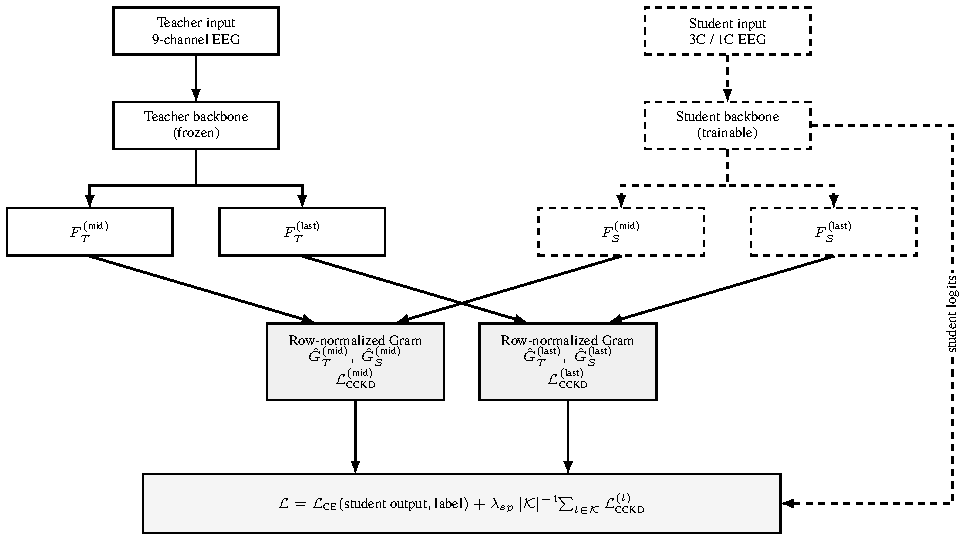
\includegraphics[width=\linewidth]{figures/method_overview.pdf}
\caption{Sơ đồ khối CCKD. Teacher cố định (xanh dương, nét liền) và student cần huấn luyện (xanh lục, nét đứt) cùng xuất đặc trưng ở lớp \texttt{mid} (đầu ra của khối tích chập không gian, sau batch normalization và hàm phi tuyến) và lớp \texttt{last} (đặc trưng áp chót, ngay trước bộ phân loại); mỗi lớp tính ma trận Gram chuẩn hóa theo hàng rồi so khớp bằng $\mathcal{L}_{\text{CCKD}}$ (đỏ). Hàm mất mát tổng cộng $\mathcal{L}$ cộng thêm cross-entropy của student.}
\label{fig:method}
\end{figure}
\FloatBarrier

Hình~\ref{fig:method} tóm tắt kiến trúc CCKD được mô tả dưới đây. Teacher nhận tín hiệu từ chín điện cực đỉnh--chẩm, được huấn luyện trước bằng cross-entropy rồi giữ cố định. Student có cùng kiến trúc với teacher nhưng chỉ nhận ba hoặc một điện cực. Với một mini-batch $N$ mẫu, gọi $F_T^{(l)} \in \mathbb{R}^{N \times d_T}$ và $F_S^{(l)} \in \mathbb{R}^{N \times d_S}$ là đặc trưng của teacher và student tại lớp $l$. Ma trận Gram của mỗi mô hình là $G^{(l)} = F^{(l)} (F^{(l)})^{\top} \in \mathbb{R}^{N \times N}$; vì ma trận Gram luôn có kích thước $N \times N$, CCKD không đòi hỏi $d_T = d_S$. Mỗi hàng được chuẩn hóa theo chuẩn $\ell_2$, $\hat{G}^{(l)}[i,:] = G^{(l)}[i,:] / \lVert G^{(l)}[i,:] \rVert_2$, và hàm mất mát quan hệ tại lớp $l$ là
\begin{equation}
\mathcal{L}_{\text{CCKD}}^{(l)} = \frac{1}{N^2} \bigl\lVert \hat{G}_{T}^{(l)} - \hat{G}_{S}^{(l)} \bigr\rVert_F^2 .
\label{eq:relloss}
\end{equation}
Với tập lớp chưng cất $\mathcal{K}$, student tối ưu $\mathcal{L} = \mathcal{L}_{\text{CE}} + \lambda_{sp} \, |\mathcal{K}|^{-1} \sum_{l \in \mathcal{K}} \mathcal{L}_{\text{CCKD}}^{(l)}$, trong đó $\mathcal{L}_{\text{CE}}$ là cross-entropy của student và $\lambda_{sp}$ là trọng số distillation. Sau huấn luyện, teacher bị loại bỏ, nên CCKD không làm thay đổi kiến trúc, số tham số hay chi phí suy luận của student \cite{R82}.

Trong công trình \cite{R82}, FB-tCNN được distill ở hai lớp, còn các kiến trúc khác chỉ ở lớp cuối, nên kiến trúc và số lớp distill bị lẫn vào nhau. Bài báo này định nghĩa hai lớp giống nhau cho mọi backbone: \textbf{lớp giữa} (\texttt{mid}, đầu ra khối tích chập không gian ngay sau chuẩn hóa batch và hàm phi tuyến, độ rộng không phụ thuộc số điện cực đầu vào) và \textbf{lớp cuối} (\texttt{last}, đặc trưng áp chót, đầu vào bộ phân loại). Giao thức chính distill chỉ lớp cuối ($\mathcal{K}=\{\texttt{last}\}$); thí nghiệm can thiệp ở Mục~\ref{sec:rq2} so sánh thêm $\mathcal{K}=\{\texttt{mid}\}$ và $\mathcal{K}=\{\texttt{mid},\texttt{last}\}$.

\subsection{Năm backbone}
\label{sec:backbones}

Bảng~\ref{tab:backbones} liệt kê năm backbone công khai dùng trong đánh giá: FB-tCNN \cite{R16}, DeepConvNet và ShallowConvNet \cite{R83}, EEGNet \cite{R84}, Compact-CNN \cite{R85}. Một số siêu tham số được điều chỉnh cho cửa sổ 1,0~s (250 mẫu ở 250~Hz): DeepConvNet giữ ba khối tích chập--pooling thay vì bốn; ShallowConvNet dùng pooling 35 mẫu, bước 7; Compact-CNN dùng kernel thời gian 64 thay vì 256.

\begin{table}[htbp]
\caption{Năm backbone và tính chất kiến trúc dùng làm biến giải thích ở RQ2. ELU: exponential linear unit, một hàm phi tuyến trơn. ``Bình phương, log'': hàm phi tuyến của ShallowConvNet bình phương đầu vào sau tích chập không gian rồi lấy log sau pooling, xấp xỉ đặc trưng công suất theo băng tần. Depthwise (tách kênh): tích chập không gian có một filter riêng cho mỗi kênh đầu vào, thay vì mỗi filter trải khắp mọi kênh (thường).}
\label{tab:backbones}
\begin{center}
\resizebox{\linewidth}{!}{%
\begin{tabular}{lccc}
\toprule
Backbone & Tích chập không gian & Hàm phi tuyến & Kernel thời gian tối đa \\
\midrule
FB-tCNN & thường, chia sẻ qua 3 băng lọc & ELU & 250 \\
DeepConvNet & thường & ELU & 10 \\
ShallowConvNet & thường & bình phương, log & 25 \\
EEGNet & depthwise & ELU & 64 \\
Compact-CNN & depthwise & ELU & 64 \\
\bottomrule
\end{tabular}}
\end{center}
\end{table}
\FloatBarrier

\subsection{Tập dữ liệu và montage}
\label{sec:data}

Hai tập dữ liệu SSVEP công khai 40 lớp mục tiêu, lấy mẫu 250~Hz: Benchmark gồm 35 subject và BETA gồm 70 subject. Mỗi cách chia subject (split) gán các subject rời nhau vào tập huấn luyện/validation/test (Benchmark: 21/4/10; BETA: 42/8/20). Tập test chỉ được đánh giá một lần. Năm split dùng seed chia 2026, 3026, 4026, 5026, 6026; mỗi split chạy tám seed khởi tạo mô hình (2026--2033).

Teacher dùng chín điện cực Pz, PO5, PO3, POz, PO4, PO6, O1, Oz, O2. Montage gốc của student là \{O1, Oz, O2\} (3C) và \{Oz\} (1C) \cite{R82}. Để trả lời RQ1b về độ nhạy montage, bài báo thêm hai montage ba điện cực \{PO3, POz, PO4\} (3C\_PPO, chỉ là nhãn montage, không liên quan tới thuật toán Proximal Policy Optimization trong học tăng cường) và \{POz, O1, O2\} (3C\_POO), cùng hai montage một điện cực \{POz\} (1C\_POz) và \{O1\} (1C\_O1), cố định trước khi chạy.

\subsection{Giao thức huấn luyện và kiểm định}
\label{sec:setup}

Mọi mô hình huấn luyện 100 epoch bằng Adam (tốc độ học $10^{-3}$, weight decay $10^{-4}$), lịch cosine annealing, batch 64; checkpoint chọn theo độ chính xác validation trung bình theo subject. Thước đo chính là độ chính xác phân loại trên subject test. Mức cải thiện $\Delta$ là chênh lệch theo cặp giữa student distill và student baseline (chỉ huấn luyện cross-entropy) trong cùng lần chạy, tính theo điểm phần trăm (pp), lấy trung bình qua seed rồi qua subject.

Với RQ1 (so sánh công bằng giữa backbone), $\lambda_{sp}=100$ được giữ cố định cho mọi backbone, dùng cùng giao thức distill-lớp-cuối thống nhất ở Mục~\ref{sec:cckd} -- khác với giao thức cũ, nơi FB-tCNN và các backbone khác không cùng số lớp distill. Với RQ1b, RQ2 và thí nghiệm can thiệp lớp, $\lambda_{sp}$ được chọn riêng cho từng cặp (dataset, backbone) theo đa số phiếu qua năm split, trong lưới ứng viên $\{1, 10, 100, 1000\}$, về giá trị nào cho độ chính xác validation tốt nhất (Bảng~\ref{tab:lambda}), để mỗi backbone được đánh giá ở mức trọng số gần tối ưu cho nó, không bị ép dùng $\lambda_{sp}=100$ nếu giá trị đó không phù hợp.

Trên một split, ý nghĩa thống kê được kiểm bằng Wilcoxon signed-rank (một kiểm định phi tham số cho cặp giá trị trước/sau) qua subject. Qua năm split, ý nghĩa được kiểm bằng kiểm định $t$ một mẫu (một kiểm định tham số so sánh trung bình mẫu với một giá trị tham chiếu cố định) trên năm giá trị $\Delta$ ($H_0$: $\bar\Delta = 0$). Khi nhiều kiểm định thuộc cùng một họ (20 tổ hợp backbone--dataset--montage ở RQ1), giá trị $p$ được hiệu chỉnh Holm--Bonferroni \cite{R86}: hiệu chỉnh này hạ ngưỡng ý nghĩa thống kê khi càng nhiều kiểm định được chạy cùng lúc, để giữ xác suất dương tính giả trên toàn họ kiểm định ở mức kiểm soát được, thay vì cộng dồn theo từng kiểm định riêng lẻ.

Với các thí nghiệm triển khai nhúng (RQ4, Mục~\ref{sec:rq4}), các ngưỡng chấp nhận và dự đoán định lượng sau được khoá trước khi đo bất kỳ số liệu RQ4 nào: lượng tử hóa sau huấn luyện giữ cùng dấu với FP32 ở ít nhất 80\% số tổ hợp có ý nghĩa ở FP32, với độ lệch cùng bậc với độ lệch chuẩn giữa các split ($\leq 0{,}5$~pp); điểm gãy độ chính xác theo độ rộng bit nằm trong khoảng 8--10 bit; thứ hạng độ trễ suy luận khớp thứ hạng dự đoán theo kernel thời gian tối đa của mỗi backbone (Bảng~\ref{tab:backbones}) ở ít nhất 4 trong 5 backbone trên cả hai board; và backbone nhỏ nhất tổng hợp được lên PL (programmable logic, phần cứng khả trình của FPGA) của ZCU104 dùng dưới 70\% LUT/DSP/Block~RAM sẵn có, với độ chính xác trên board trong 1~pp so với mô phỏng bit-chính-xác H2.

\begin{table}[htbp]
\caption{$\lambda_{sp}$ theo đa số phiếu trên validation (5 split), dùng cho RQ1b, RQ2 và thí nghiệm can thiệp lớp.}
\label{tab:lambda}
\begin{center}
\begin{tabular}{lccccc}
\toprule
Dataset & FB-tCNN & DeepConvNet & EEGNet & ShallowConvNet & Compact-CNN \\
\midrule
Benchmark & 100 & 100 & 10 & 10 & 10 \\
BETA & 100 & 1000 & 10 & 100 & 10 \\
\bottomrule
\end{tabular}
\end{center}
\end{table}

\section{Kết quả và Thảo luận}

\subsection{RQ1: mức cải thiện theo backbone ở trọng số cố định}
\label{sec:rq1}

Bảng~\ref{tab:rq1} tổng hợp mức cải thiện của CCKD trên năm backbone, hai tập dữ liệu và hai montage, ở $\lambda_{sp}=100$ cố định và giao thức distill-lớp-cuối thống nhất cho mọi backbone (20 tổ hợp, mỗi tổ hợp 5 split $\times$ 8 seed).

Trong 20 tổ hợp, 5 cải thiện có ý nghĩa và 4 suy giảm có ý nghĩa trước hiệu chỉnh; sau Holm--Bonferroni, chỉ 2 tổ hợp còn ý nghĩa, cả hai đều âm (EEGNet trên BETA, cả 3C và 1C). Kết quả không xếp được theo nhóm kiến trúc: FB-tCNN và DeepConvNet có xu hướng cải thiện (dương ở 3/4 và 4/4 thiết lập), ShallowConvNet suy giảm trên Benchmark nhưng cải thiện trên BETA, còn EEGNet đổi dấu giữa hai tập dữ liệu (cải thiện trên Benchmark, suy giảm có ý nghĩa mạnh trên BETA). Điều này cho thấy kết luận trước đó rằng CCKD cải thiện FB-tCNN \cite{R82} không khái quát được cho CCKD nói chung; mức cải thiện phụ thuộc vào cả backbone và tập dữ liệu.

\begin{table}[htbp]
\caption{Mức cải thiện CCKD qua 5 split ($\lambda_{sp}=100$ cho mọi backbone, distill lớp cuối). Montage student: 3C $=\{$O1, Oz, O2$\}$ (3 điện cực), 1C $=\{$Oz$\}$ (1 điện cực). Mỗi ô: $\bar\Delta$ (pp) và $p$ của kiểm định $t$ một mẫu qua split. \textbf{Đậm}: $p<0.05$ (chưa hiệu chỉnh). $^\dagger$: còn ý nghĩa sau hiệu chỉnh Holm--Bonferroni trên cả 20 kiểm định ($p_{\text{Holm}}<0.05$).}
\label{tab:rq1}
\begin{center}
\footnotesize
\begin{tabular}{lcccc}
\toprule
Backbone & Benchmark 3C & Benchmark 1C & BETA 3C & BETA 1C \\
\midrule
FB-tCNN & \textbf{+0.78 (0.0043)} & +0.25 (0.138) & \textbf{+1.09 (0.0075)} & $-0.15$ (0.658) \\
DeepConvNet & +0.36 (0.050) & \textbf{+0.14 (0.025)} & \textbf{+0.49 (0.023)} & +0.60 (0.065) \\
EEGNet & +0.98 (0.094) & $-0.36$ (0.310) & \textbf{$-1.33$ (0.0008)}$^\dagger$ & \textbf{$-1.33$ (0.0017)}$^\dagger$ \\
ShallowConvNet & \textbf{$-0.75$ (0.043)} & \textbf{$-1.01$ (0.011)} & +0.44 (0.278) & \textbf{+0.49 (0.034)} \\
Compact-CNN & +0.18 (0.646) & $-0.43$ (0.124) & $-0.16$ (0.485) & $-0.15$ (0.221) \\
\bottomrule
\end{tabular}
\end{center}
\end{table}

Hai tổ hợp còn ý nghĩa sau hiệu chỉnh Holm--Bonferroni đều được đo ở $\lambda_{sp}=100$, mức cố định dùng cho so sánh liên-backbone ở trên; $\lambda_{sp}$ tối ưu riêng của EEGNet theo validation là 10 (Bảng~\ref{tab:lambda}). Ở mức $\lambda_{sp}$ tối ưu này, tính trên cùng 5 split, cả hai tổ hợp đều không còn ý nghĩa và đổi dấu (BETA 3C: $\bar\Delta=+0,11$~pp, $p=0,368$; BETA 1C: $\bar\Delta=+0,03$~pp, $p=0,704$). Rộng hơn, trong 12 tổ hợp có $\lambda_{sp}$ tối ưu khác 100, kết luận có-ý-nghĩa/không ($p<0,05$, chưa hiệu chỉnh) đổi chiều giữa mức cố định và mức tối ưu ở 5 trên 12 tổ hợp, theo cả hai hướng. Không có tổ hợp nào trong nghiên cứu này vừa còn ý nghĩa sau hiệu chỉnh ở mức $\lambda_{sp}$ cố định dùng cho RQ1 vừa còn ý nghĩa ở mức $\lambda_{sp}$ tối ưu riêng của nó: hiệu ứng duy nhất còn lại sau hiệu chỉnh ở đây thực chất là do đánh giá backbone đó lệch khỏi điểm vận hành tối ưu của chính nó, không phải một tính chất của kiến trúc độc lập với siêu tham số.

Để kiểm tra độ bền vững của kiểm định $t$ một mẫu bằng một kiểm định phi tham số, chúng tôi lặp lại cả 20 kiểm định bằng Wilcoxon signed-rank và bằng kiểm định hoán vị đổi dấu (sign-flip) chính xác trên năm giá trị $\Delta$ theo split. Với chỉ năm split, giá trị $p$ hai phía nhỏ nhất mà một trong hai kiểm định phi tham số chính xác này có thể cho ra là $2/2^5=0{,}0625$, bất kể độ lớn hiệu ứng: đây là một tính chất tổ hợp của $n=5$, không phải một ước lượng power riêng cho dữ liệu này. Vì hiệu chỉnh Holm--Bonferroni trên 20 kiểm định đòi hỏi giá trị $p$ danh nghĩa nhỏ nhất phải dưới $0{,}05/20=0{,}0025$, không kiểm định nào trong họ này có thể còn ý nghĩa sau hiệu chỉnh bằng một trong hai phương pháp phi tham số, dù hiệu ứng thật có lớn đến đâu. Hai ô còn ý nghĩa sau hiệu chỉnh nêu trên vì vậy phụ thuộc cụ thể vào giả định của kiểm định $t$ một mẫu rằng các giá trị $\Delta$ theo split xấp xỉ phân phối chuẩn, một giả định không thể kiểm chứng đáng tin cậy ở cùng cỡ mẫu này; hạn chế mang tính cấu trúc của thiết kế $n=5$ này nên được cân nhắc cùng với độ nhạy $\lambda_{sp}$ ở trên khi đánh giá kết quả còn lại duy nhất này đáng tin đến mức nào.

\subsection{RQ1b: độ nhạy theo montage}
\label{sec:rq1b}

Bảng~\ref{tab:rq1b} so sánh mức cải thiện ở montage gốc với hai montage thay thế cho mỗi cấu hình 3C/1C, ở $\lambda_{sp}$ chọn theo Bảng~\ref{tab:lambda} (40 tổ hợp thay thế).

Đổi montage student sang một tập con điện cực khác làm đảo dấu hiệu ứng trong 12 trên 40 trường hợp. Dấu hiệu bị đảo xuất hiện ở cả hai hướng (từ có lợi thành không có lợi và ngược lại) và không tập trung vào một backbone hay một dataset cụ thể, dù ShallowConvNet và Compact-CNN có tỷ lệ đảo dấu cao hơn. Các so sánh montage này không được kiểm định ý nghĩa thống kê riêng, và phần lớn mức đảo dấu nhỏ: 11 trong 12 trường hợp có độ lớn dưới 0,3~pp, thấp hơn độ lệch chuẩn giữa các split trung vị 0,48~pp của $\Delta$ quan sát được trên 20 tổ hợp RQ1 (Bảng~\ref{tab:rq1}), nên tỷ lệ đảo dấu thật sự vượt quá nhiễu đo là thấp hơn con số thô này gợi ý. Điều này cho thấy lợi ích của CCKD nhạy với vị trí điện cực, không chỉ với số điện cực, dù việc xác nhận độ nhạy này bằng kiểm định ý nghĩa thống kê riêng ở các montage thay thế còn để lại cho nghiên cứu sau.

\begin{table}[htbp]
\caption{Mức cải thiện ($\bar\Delta$, pp, qua 5 split) ở montage gốc so với hai montage thay thế mỗi cấu hình, tất cả ở $\lambda_{sp}$ tối ưu riêng từng backbone theo validation (Bảng~\ref{tab:lambda}). $^\star$: đổi dấu so với montage gốc. Montage 3 điện cực: Gốc $=\{$O1, Oz, O2$\}$, PPO $=\{$PO3, POz, PO4$\}$, POO $=\{$POz, O1, O2$\}$. Montage 1 điện cực: Gốc $=\{$Oz$\}$, POz $=\{$POz$\}$, O1 $=\{$O1$\}$. Do đó cột "Gốc" không trùng với các giá trị $\lambda_{sp}=100$ cố định ở Bảng~\ref{tab:rq1} với những backbone có mức tối ưu khác 100.}
\label{tab:rq1b}
\begin{center}
\footnotesize
\begin{tabular}{lcccccc}
\toprule
 & \multicolumn{3}{c}{3 điện cực} & \multicolumn{3}{c}{1 điện cực} \\
Backbone & Gốc & PPO & POO & Gốc & POz & O1 \\
\midrule
\multicolumn{7}{l}{\textit{Benchmark}} \\
FB-tCNN & +0.78 & +0.24 & +0.70 & +0.25 & $-0.09^\star$ & +0.83 \\
DeepConvNet & +0.36 & +0.20 & +0.02 & +0.14 & +0.20 & +0.81 \\
EEGNet & +1.60 & +1.14 & +0.64 & +0.51 & +0.92 & $-0.06^\star$ \\
ShallowConvNet & $-0.15$ & +0.09$^\star$ & $-0.18$ & $-0.42$ & $-0.30$ & +0.05$^\star$ \\
Compact-CNN & +0.26 & $-0.11^\star$ & +0.31 & $-0.17$ & +0.29$^\star$ & +0.04$^\star$ \\
\multicolumn{7}{l}{\textit{BETA}} \\
FB-tCNN & +1.09 & +0.54 & +1.10 & $-0.15$ & +0.17$^\star$ & +0.43$^\star$ \\
DeepConvNet & +0.93 & +1.34 & +0.80 & +1.12 & +1.10 & +1.68 \\
EEGNet & +0.11 & +0.24 & +0.02 & +0.03 & $-0.17^\star$ & +0.18 \\
ShallowConvNet & +0.44 & +0.65 & +0.13 & +0.49 & +0.04 & +0.61 \\
Compact-CNN & +0.01 & $-0.03^\star$ & +0.14 & +0.16 & $-0.00^\star$ & +0.03 \\
\bottomrule
\end{tabular}
\end{center}
\end{table}

\subsection{RQ2: đại lượng dự đoán mức cải thiện}
\label{sec:rq2}

\subsubsection{Độ tương đồng CKA giữa teacher và student}

Hàm mất mát~\eqref{eq:relloss} kéo ma trận Gram của student về phía ma trận Gram của teacher; nếu CCKD có ích bằng cơ chế này, mức cải thiện độ chính xác phải đi cùng mức tăng CKA. CKA tuyến tính được đo giữa đặc trưng lớp cuối của teacher và student trên tập test, ở $\lambda_{sp}$ theo Bảng~\ref{tab:lambda}. Ký hiệu $\Delta$CKA là CKA của student distill trừ CKA của student baseline, trung bình qua 5 split và 8 seed.

Trên 20 tổ hợp, $\Delta$CKA tương quan với $\bar\Delta$ (Pearson $r=0.55$, hệ số tương quan tuyến tính, mức tương quan dương trung bình-đến-mạnh, $p=0.012$; Spearman $\rho=0.57$, hệ số tương quan hạng, $p=0.009$), xem Hình~\ref{fig:rq2a}. CKA của student baseline (trước distillation) không tương quan với mức cải thiện (Pearson $r=-0.11$, $p=0.65$; Spearman $\rho=-0.03$, $p=0.91$). Như vậy, mức chênh biểu diễn ban đầu giữa teacher và student không dự đoán được hiệu quả của CCKD; điều dự đoán được là \emph{mức CCKD thu hẹp chênh lệch đó}, phù hợp với cơ chế của hàm mất mát. 20 điểm này không hoàn toàn độc lập: mỗi backbone đóng góp bốn điểm (hai dataset $\times$ hai montage) cùng chung kiến trúc, nên tương quan và giá trị $p$ danh nghĩa này mô tả xu hướng chung giữa các tổ hợp hơn là một kiểm định với 20 bậc tự do độc lập. Một kiểm định hoán vị theo cụm, giữ nguyên cách nhóm này -- hoán vị xem bốn giá trị $\Delta$CKA của backbone nào ghép với bốn giá trị $\bar\Delta$ của backbone nào, đủ cả $5!=120$ cách gán -- cho $p=0,025$: tương quan vẫn còn ý nghĩa dưới suy luận đúng mức cụm, dù ở mức thận trọng hơn so với $p=0,012$ ngây thơ ở trên. Tính tương quan chỉ trên năm điểm trung bình theo backbone loại bỏ hết biến thiên trong-backbone và tương ứng thiếu power ($r=0,74$, $p=0,15$, $n=5$); điều này phản ánh việc chỉ có năm cụm backbone ngay từ đầu, không phải bằng chứng phản bác mối liên hệ này.

\begin{figure}[htbp]
\centering
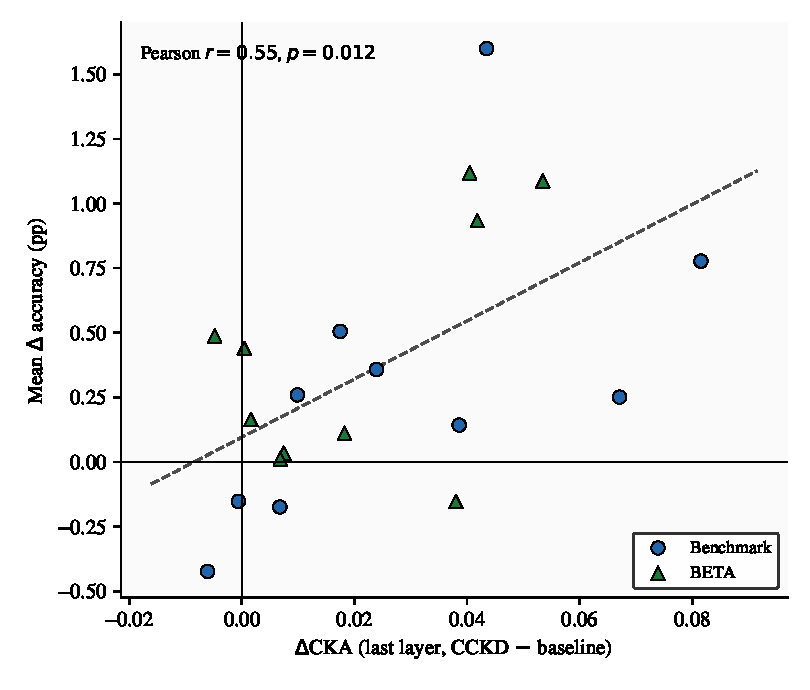
\includegraphics[width=0.62\linewidth]{figures/rq2a_scatter.pdf}
\caption{Mức tăng CKA lớp cuối do CCKD gây ra so với mức cải thiện độ chính xác, 20 tổ hợp backbone--dataset--montage. Đường đứt: hồi quy tuyến tính. Hình tròn: Benchmark; tam giác: BETA.}
\label{fig:rq2a}
\end{figure}

\subsubsection{Thí nghiệm can thiệp theo lớp distill}
\label{sec:layer_intervention}

Tương quan ở trên chỉ mang tính quan sát: nó không chứng minh mức tăng CKA gây ra mức cải thiện độ chính xác, vì cả hai có thể cùng phụ thuộc vào một tính chất khác của kiến trúc. Như một so sánh thực nghiệm riêng, chúng tôi thay đổi tập lớp distill $\mathcal{K} \in \{\texttt{last}, \texttt{mid}, \{\texttt{mid},\texttt{last}\}\}$ để kiểm tra lớp nào cho mức cải thiện lớn hơn, trong khi giữ nguyên backbone, dataset, montage và $\lambda_{sp}$.

Trên 20 tổ hợp: distill riêng lớp cuối cho mức cải thiện lớn hơn distill riêng lớp giữa chỉ trong 5 tổ hợp, nên distill riêng lớp giữa đạt bằng hoặc vượt giao thức distill-lớp-cuối ở 15 trong 20 tổ hợp. Nói cách khác, lựa chọn lớp của giao thức chính (distill lớp cuối \cite{R82}) thường không phải là lựa chọn tốt nhất. Distill đồng thời cả hai lớp là một phép so sánh khác, chặt hơn: nó đạt bằng hoặc vượt lựa chọn một-lớp tốt hơn chỉ trong 8 trên 20 tổ hợp, nên kết hợp hai lớp thường không phải là lựa chọn tốt nhất; đây là kết quả thiểu số, dù không bao giờ cần biết trước lớp nào sẽ thắng nếu chỉ dùng một lớp. Độ chính xác và $\Delta$CKA chi tiết theo từng tổ hợp tại lớp được distill nằm trong kho mã nguồn đi kèm bài báo (xem mục Khả năng tái lập).

\subsection{RQ3: độ tin cậy của đánh giá một-split so với nhiều-split}
\label{sec:rq3}

Bảng~\ref{tab:rq3} so sánh kết luận rút ra từ một split (2026, kiểm định Wilcoxon qua subject) với kết luận từ năm split (kiểm định $t$ qua split), cho 20 tổ hợp ở $\lambda_{sp}=100$ (giao thức RQ1).

Đánh giá trên một split đánh giá sai dấu hoặc ý nghĩa thống kê của hiệu ứng trong 10 trên 20 tổ hợp -- đúng một nửa. Sai lệch xảy ra theo cả hai chiều: một split có thể bỏ sót một cải thiện hoặc suy giảm ổn định (ví dụ FB-tCNN Benchmark-3C, DeepConvNet 1C ở cả hai tập dữ liệu), hoặc báo cáo một hiệu ứng không lặp lại khi dùng nhiều split (ví dụ ShallowConvNet BETA-3C). Hai kiểm định không cùng đơn vị lặp (Wilcoxon lặp qua subject, kiểm định $t$ lặp qua split), nên bảng không cho biết kiểm định nào có công suất thống kê cao hơn; điều bảng cho thấy là một nghiên cứu chỉ báo cáo một split có thể đi đến kết luận ngược với kết luận khi lặp lại trên các tập subject khác, ở mức hiệu ứng điển hình của tài liệu CCKD cho SSVEP (dưới 1--2~pp).

\begin{table}[htbp]
\caption{Kết luận trên một split (2026) so với năm split, $\lambda_{sp}=100$. $+$/$-$/$0$: cải thiện/suy giảm/không có ý nghĩa ($p<0.05$). $^\star$: kết luận khác nhau (dấu hoặc ý nghĩa thống kê). Montage student: 3C $=\{$O1, Oz, O2$\}$ (3 điện cực), 1C $=\{$Oz$\}$ (1 điện cực).}
\label{tab:rq3}
\begin{center}
\footnotesize
\begin{tabular}{llcccc}
\toprule
Backbone & Student & Một split (pp, $p$) & Năm split (pp, $p$) & Benchmark & BETA \\
\midrule
FB-tCNN & 3C & $+0.31$ (0.359) & $+0.78$ (0.0043) & $0 \to +$ $^\star$ & $0 \to +$ $^\star$ \\
 & 1C & $+0.22$ (0.447) & $+0.25$ (0.138) & $0 \to 0$ & $0 \to 0$ \\
DeepConvNet & 3C & $+0.17$ (0.492) & $+0.36$ (0.050) & $0 \to 0$ & $+ \to +$ \\
 & 1C & $+0.01$ (0.980) & $+0.14$ (0.025) & $0 \to +$ $^\star$ & $0 \to 0$ $^\star$ \\
EEGNet & 3C & $-0.20$ (0.770) & $+0.98$ (0.094) & $0 \to 0$ $^\star$ & $- \to -$ \\
 & 1C & $+0.32$ (0.557) & $-0.36$ (0.310) & $0 \to 0$ $^\star$ & $- \to -$ \\
ShallowConvNet & 3C & $-0.52$ (0.322) & $-0.75$ (0.043) & $0 \to -$ $^\star$ & $0 \to 0$ \\
 & 1C & $-0.67$ (0.041) & $-1.01$ (0.011) & $- \to -$ & $+ \to +$ \\
Compact-CNN & 3C & $-0.15$ (0.820) & $+0.18$ (0.646) & $0 \to 0$ $^\star$ & $0 \to 0$ $^\star$ \\
 & 1C & $-0.97$ (0.014) & $-0.43$ (0.124) & $- \to 0$ $^\star$ & $0 \to 0$ \\
\bottomrule
\end{tabular}
\end{center}
\end{table}

\subsection{RQ4: triển khai nhúng}
\label{sec:rq4}

Mục này dùng bốn sơ đồ lượng tử hóa/số học cố định khác nhau, mỗi thí nghiệm con một sơ đồ, vì mỗi
thí nghiệm nhắm vào một tính chất khác nhau (giữ độ chính xác, độ nhạy theo độ rộng bit qua mô
phỏng, độ trễ CPU, tổng hợp FPGA) và không sơ đồ nào thỏa ràng buộc của cả bốn công cụ cùng lúc;
chúng không được đánh giá chung như một sản phẩm triển khai duy nhất, mỗi sơ đồ được nêu rõ tên bên
dưới. Chúng tôi lượng tử hóa sau huấn luyện tĩnh (static post-training quantization, PTQ) sang INT8 cho
mô hình student đã huấn luyện ở RQ1, chỉ đánh giá lại trên tập test, không huấn luyện lại. Ở 2 tổ
hợp backbone--dataset--montage còn ý nghĩa thống kê sau hiệu chỉnh Holm--Bonferroni (RQ1, cả hai
trên EEGNet với BETA, montage 3C và 1C), độ lệch độ chính xác do PTQ gây ra giữ cùng dấu với FP32
trong toàn bộ 10/10 tổ hợp split--seed (100\%) và không vượt quá 0,26~pp, nhỏ hơn độ lệch chuẩn giữa
các split điển hình của $\Delta$ trên 20 tổ hợp RQ1 (trung vị 0,48~pp, khoảng tứ phân vị 0,31--0,69~pp,
tính từ các giá trị $sd_{pp}$ theo từng tổ hợp làm nền cho Bảng~\ref{tab:rq1}).

Chúng tôi tiếp tục quét độ rộng số học cố định (fixed-point) $\{16,12,10,8\}$ bit bằng mô phỏng
bit-chính-xác (bit-accurate) của hls4ml cho EEGNet và DeepConvNet, backbone nhỏ nhất và lớn nhất
theo số tham số thật (EEGNet: 5.640--5.672 tham số; DeepConvNet: 99.940--101.190 tham số tùy montage,
so với 44.488--90.536 của ba backbone còn lại), trên tập BETA với 5 split. Độ chính xác của EEGNet giữ trong 1~pp của FP32 ở
độ rộng 10 bit trở lên và giảm hơn 4~pp dưới 8 bit ở cả hai montage, đúng vùng điểm gãy 8--10 bit dự
kiến trước khi đo. DeepConvNet (montage 3C) giữ gần như không đổi ở 10--16 bit (lệch dưới 0,05~pp)
nhưng giảm mạnh dưới 8 bit (lệch 1,5~pp ở 8 bit, 20,4~pp ở 6 bit, quét thêm quanh điểm gãy theo đúng
phạm vi đã khóa trước), cho thấy điểm gãy thật nằm giữa 6 và 8 bit, thấp hơn khoảng dự kiến một mức.

Chúng tôi đo độ trễ suy luận của cả 5 backbone ở FP32 và INT8 trên Raspberry Pi 4 (Cortex-A72) và
lõi xử lý (processing system, PS) Cortex-A53 của Xilinx ZCU104, mỗi cấu hình lấy trung bình trên 7
tiến trình độc lập, 100 lần suy luận mỗi tiến trình, batch 1, cửa sổ 1,0~s; đây là các đợt đo ngắn, chạy một tiến trình, nên số liệu báo cáo đặc trưng cho chế độ này, không đặc trưng cho vận hành liên tục theo chu kỳ (thermal throttling, các tiến trình vòng điều khiển chạy đồng thời, hay hiệu ứng khi chạy pin trong thời gian dài). Ở đây INT8 dùng lượng tử
hóa động theo trọng số (dynamic quantization, chỉ lượng tử hóa trọng số lớp tích chập/tuyến tính,
kích hoạt vẫn ở FP32): lượng tử hóa tĩnh báo lỗi không tương thích với kernel lượng tử hóa cho các
toán tử ELU và bình phương dùng trong FB-tCNN, DeepConvNet và ShallowConvNet, xác nhận giống nhau
trên cả hai board; EEGNet và Compact-CNN cũng dùng ELU nhưng kết hợp với tích chập tách kênh
(depthwise) thay vì tích chập thường, lại không gặp lỗi này, nên nhiều khả năng tích chập thường
(không phải riêng hàm phi tuyến) mới là yếu tố phân biệt thật. Ở độ rộng INT8, toàn bộ 5 backbone có
độ trễ suy luận thuần (forward pass) dưới 16~ms trên cả hai board, kể cả cộng thêm thời gian lọc
băng tần (filter bank) của FB-tCNN (tổng pipeline tối đa 24,5~ms trên ZCU104 PS). Độ trễ tính toán
thuần này thấp hơn một ngân sách vòng điều khiển minh họa 300~ms khoảng 12 lần; ngân sách này chỉ là
giả định, không có nguồn từ một bộ điều khiển xe lăn hay bộ đánh vần cụ thể, và chưa tính cửa sổ
kích thích SSVEP 1,0~s mà cùng giao thức yêu cầu trước khi có được đoạn tín hiệu này, nên chỉ giới
hạn phần đóng góp của riêng bộ phân loại vào khâu trễ của vòng điều khiển, không phải toàn bộ độ trễ
từ quyết định tới tác động. Trên PS của ZCU104, công suất board đo qua cảm biến INA226 có sẵn trên
board tăng từ mức nền khi rảnh 11,75~W lên 12,32--12,45~W khi suy luận liên tục, tức tăng thêm
0,61--0,76~W do suy luận trên cả 5 backbone ở cả FP32 và INT8, không thấy khác biệt rõ theo độ rộng
số học. Không báo cáo số liệu tương ứng trên Raspberry Pi 4: board loại thường (stock) không có cảm
biến công suất hay dòng điện lộ ra cho phần mềm (\texttt{vcgencmd pmic\_read\_adc} không trả về rail
nào đã đăng ký trên firmware này), nên công suất ở mức board chỉ báo cáo trên ZCU104. Bảng~\ref{tab:rq4latency} liệt kê độ trễ pipeline tổng theo từng backbone, từng board, từng độ rộng số học, là số liệu nền cho các con số trên và cho phần xếp hạng bàn tiếp theo.

Thứ hạng độ trễ đo được (từ nhanh đến chậm: ShallowConvNet, EEGNet, DeepConvNet, Compact-CNN,
FB-tCNN) giống nhau trên cả hai board nhưng không khớp thứ hạng dự kiến theo kernel thời gian tối đa
của mỗi backbone (Bảng~\ref{tab:backbones}) hay theo số phép tính dấu phẩy động (FLOPs) đo trực
tiếp để thay thế đại diện đó: chỉ 2/5 vị trí khớp theo kernel và 3/5 vị trí khớp theo FLOPs, cả hai
dưới ngưỡng đa số (4/5) đặt trước khi đo -- một phép kiểm thô vì chỉ có 5 vị trí xếp hạng khả dĩ. Hệ số tương quan hạng cho một góc nhìn bổ sung, bớt kiểu tất-cả-hoặc-không-gì, ở cùng cỡ mẫu nhỏ này (Spearman $\rho$, $n=5$, giá trị $p$ chỉ mang tính tham khảo): $\rho=0,62$ cho xếp hạng theo kernel và $\rho=0,90$ cho xếp hạng theo FLOPs.
Sai lệch tập trung ở hai backbone nhanh nhất: EEGNet có
FLOPs thấp nhất (0,87 triệu FLOPs tại montage 3C) nhờ tích chập tách kênh (depthwise/separable
convolution) nhưng đo được chậm hơn ShallowConvNet (4,03 triệu FLOPs) một chút trên cả hai board, một phép hoán vị liền kề ở đầu bảng xếp hạng, lý giải vì sao hệ số tương quan theo FLOPs cao dù không đạt ngưỡng đa số về vị trí khớp chính xác,
cho thấy ở quy mô mô hình rất nhỏ này, chi phí thực thi trên CPU ARM không tỉ lệ thuận với số tham
số, kernel hay FLOPs lý thuyết, dù FLOPs vẫn bám sát xếp hạng chung hơn là con số khớp-vị-trí-chính-xác cho thấy.

\begin{table}[htbp]
\caption{Độ trễ pipeline tổng (ms, trung bình trên 7 tiến trình $\times$ 100 lần suy luận, batch 1), đã cộng bước lọc băng tần cho FB-tCNN. Pi4: Raspberry Pi 4 (Cortex-A72). ZCU104: PS Cortex-A53.}
\label{tab:rq4latency}
\begin{center}
\footnotesize
\begin{tabular}{lcccc}
\toprule
 & \multicolumn{2}{c}{Pi4} & \multicolumn{2}{c}{ZCU104 PS} \\
Backbone & FP32 & INT8 & FP32 & INT8 \\
\midrule
FB-tCNN & 13,5 & 13,4 & 24,4 & 24,5 \\
DeepConvNet & 3,9 & 3,5 & 5,5 & 5,3 \\
ShallowConvNet & 2,8 & 2,6 & 4,0 & 4,0 \\
EEGNet & 3,1 & 3,1 & 4,6 & 4,8 \\
Compact-CNN & 6,0 & 5,9 & 9,2 & 9,4 \\
\bottomrule
\end{tabular}
\end{center}
\end{table}

Chúng tôi tổng hợp EEGNet (montage 1C, BETA split 2026/seed 2026, student CCKD $\lambda_{sp}=100$,
độ rộng 10 bit) lên PL (programmable logic, phần cứng khả trình của FPGA) của ZCU104. Cấu hình này là
một trong hai tổ hợp (EEGNet, BETA, montage 3C và 1C) mà CCKD làm suy giảm có ý nghĩa thống kê sau
hiệu chỉnh Holm--Bonferroni (RQ1, Bảng~\ref{tab:rq1}), được đo ở đây tại một split và một seed duy
nhất (2026/2026, split đầu tiên và seed khởi tạo mô hình đầu tiên theo thứ tự đặt trước dùng xuyên suốt bài báo này, Mục~\ref{sec:data}, khóa trước khi thấy bất kỳ kết quả phần cứng nào) thay vì lấy trung bình trên năm split như những phần khác của bài báo; vì vậy phép đo
trên board dưới đây kiểm tra việc triển khai phần cứng có tái tạo đúng mô phỏng bit-chính-xác của chính nó hay không, chứ không kiểm tra CCKD có lợi ở tổ hợp này hay không; phép đo này cũng dùng lại đúng datapath số học đã tổng hợp bằng HLS từ lần thử AXI-Stream trước đó (đã bỏ), chỉ phần giao diện cấp cao nhất thay đổi, nên việc khớp sát với mô phỏng là một phép kiểm chặt cho riêng giao diện và logic chuyển dữ liệu, không phải một lần tái dựng độc lập cho lõi tính toán fixed-point. Lần đầu dùng
\texttt{hls4ml}, một công cụ dịch mạng đã huấn luyện thành đặc tả phần cứng số học cố định
bit-chính-xác để mô phỏng và tổng hợp, qua backend VivadoAccelerator của nó (AXI-Stream và AXI DMA,
một giao diện truyền dữ liệu dạng luồng có tín hiệu đóng khung/bắt tay riêng); hướng này tổng hợp và
sinh bitstream được, nhưng gặp lỗi dai dẳng ở tín hiệu TLAST (tín hiệu đánh dấu từ cuối cùng của một
lần truyền dữ liệu) trên cổng ra, không hết sau sáu lượt sửa lỗi khác nhau của thư viện, nên không
dùng được trên board thật. Vì vậy chúng tôi bọc lại chính kernel suy luận đã kiểm chứng đó bằng giao
diện AXI ánh xạ bộ nhớ (m\_axi) viết tay cùng một thanh ghi điều khiển AXI-Lite, một giao diện dạng
thanh ghi đơn giản hơn tránh hẳn vấn đề đóng khung của AXI-Stream; Vitis HLS và Vivado 2024.2 tổng
hợp, triển khai (place and route) và sinh bitstream đều thành công ở xung nhịp 100~MHz, timing đóng
với biên dư 2,074~ns. Tài nguyên toàn thiết kế (lõi xử lý Zynq và IP suy luận) dùng 11,75\% bảng tra
cứu (LUT), 6,54\% flip-flop (FF), 9,13\% số khối BRAM, và 96 trên 1728 khối DSP48E2 (5,56\%) của board
XCZU7EV, dưới xa ngưỡng 70\% đã khoá trước (Mục~\ref{sec:setup}). Độ trễ đầu-cuối, tính
bằng tổng thời gian thực đo trên 3200 lần suy luận liên tiếp chia cho số cửa sổ (gồm cả thời gian ghi
thanh ghi AXI-Lite, vòng lặp chờ cờ hoàn tất phía host, và đóng gói dữ liệu của PYNQ, không chỉ chu kỳ
tính toán nội bộ của FPGA), là 1,17~ms mỗi cửa sổ. Chúng tôi nạp bitstream này lên ZCU104 và chạy suy
luận trên toàn bộ 3200 cửa sổ test thật của BETA cho cấu hình này: độ chính xác trên board là
24,06\%, so với 24,09\% của mô phỏng bit-chính-xác H2 ở cùng độ rộng 10 bit, chênh lệch 0,03~pp, nằm
rất sâu trong ngưỡng 1~pp đã khoá trước (Mục~\ref{sec:setup}). Để đối chiếu, độ chính xác baseline
(chưa distill) của chính tổ hợp này là 25,35\%, gần cận dưới của khoảng 22,50--55,83\% độ chính xác
baseline trên toàn bộ 20 tổ hợp backbone--dataset--montage trong bài báo, phù hợp với hiệu ứng làm
suy giảm của CCKD ở tổ hợp này (RQ1). Công suất board khi suy luận liên tục (10,45--10,50~W) không
cao hơn rõ rệt mức nền khi rảnh (10,55~W) ở độ phân giải của cảm biến INA226 trên board, phù hợp với
mức sử dụng tài nguyên thấp của thiết kế PL này.

Bảng~\ref{tab:deploysummary} gom lại các số liệu accuracy và độ trễ nằm rải rác trong mục này cho đúng một cấu hình (EEGNet, BETA, montage 1C, $\lambda_{sp}=100$), tổ hợp duy nhất đi hết đến bước kiểm phần cứng thật, để người đọc không phải tự ghép lại từ các đoạn văn ở trên. Mỗi hàng ghi rõ chế độ đo, vì chúng không cùng cách tính: các hàng accuracy đánh dấu ``lần chạy này'' là số liệu một split, một seed (2026/2026) riêng cho phép kiểm phần cứng; hàng mức cải thiện CCKD là trung bình 5 split trên toàn nghiên cứu lấy từ Bảng~\ref{tab:rq1}, không so sánh trực tiếp được về độ lớn với các hàng accuracy một-lần-chạy; còn hàng độ trễ và công suất PS đo bằng phần mềm trên lõi ARM (Mục~\ref{sec:setup}), khác chế độ với hàng PL đo trên phần cứng tổng hợp.

\begin{table}[htbp]
\caption{Accuracy, độ trễ và công suất cho đúng một cấu hình đã đi tới bước phần cứng (EEGNet, BETA, montage 1C, $\lambda_{sp}=100$), gom lại các số liệu đã báo riêng lẻ trong mục này. PS: suy luận bằng phần mềm trên lõi ARM. PL: bộ tăng tốc phần cứng đã tổng hợp.}
\label{tab:deploysummary}
\begin{center}
\footnotesize
\begin{tabular}{llc}
\toprule
Đại lượng & Chế độ & Giá trị \\
\midrule
Độ chính xác baseline (chưa distill) & FP32, lần chạy này & 25,35\% \\
Mức cải thiện CCKD (trung bình 5 split) & FP32, Bảng~\ref{tab:rq1} & $-1,33$ pp \\
Độ chính xác mô phỏng bit-chính-xác (10 bit) & H2, lần chạy này & 24,09\% \\
Độ chính xác trên board & ZCU104 PL, lần chạy này & 24,06\% \\
Độ trễ pipeline tổng, INT8 & Pi4 PS, Bảng~\ref{tab:rq4latency} & 3,1 ms \\
Độ trễ pipeline tổng, INT8 & ZCU104 PS, Bảng~\ref{tab:rq4latency} & 4,8 ms \\
Độ trễ đầu-cuối & ZCU104 PL, lần chạy này & 1,17 ms \\
Công suất, suy luận $-$ rảnh & ZCU104 PS, cả 5 backbone & $+0,61$ đến $+0,76$ W \\
Công suất, suy luận $-$ rảnh & ZCU104 PL, lần chạy này & không đo được khác biệt \\
\bottomrule
\end{tabular}
\end{center}
\end{table}

\section{Kết luận}

CCKD không mang lại lợi ích nhất quán khi mở rộng từ FB-tCNN sang bốn backbone khác: trong 20 tổ hợp backbone--dataset--montage đánh giá ở trọng số cố định chung cho mọi backbone, chỉ 2 còn ý nghĩa thống kê sau hiệu chỉnh cho so sánh đa biến, và cả hai đều là suy giảm; không tổ hợp nào còn giữ ý nghĩa ở $\lambda_{sp}$ tối ưu riêng của chính backbone đó, nên không có tổ hợp nào trong nghiên cứu này vừa có ý nghĩa sau hiệu chỉnh vừa bền vững trước lựa chọn trọng số distillation (RQ1). Lợi ích của CCKD, khi có, nhạy với việc chọn montage cụ thể, không chỉ với số điện cực (RQ1b). Mức tăng CKA do distillation gây ra tương quan với mức cải thiện độ chính xác qua các backbone, nhưng tương quan này chỉ mang tính quan sát và mức chênh CKA trước distillation thì không dự đoán được mức cải thiện; trong ba lựa chọn lớp distill đã kiểm, distill riêng lớp giữa thường đạt bằng hoặc vượt giao thức distill-lớp-cuối \cite{R82} (15 trên 20 tổ hợp), nhưng kết hợp cả hai lớp cũng thường không phải lựa chọn tốt nhất (8 trên 20 tổ hợp) (RQ2). Đánh giá trên một split subject, giao thức phổ biến trong tài liệu KD cho EEG, đánh giá sai dấu hoặc ý nghĩa thống kê của hiệu ứng ở một nửa số tổ hợp (RQ3). Hiệu ứng độ chính xác của mô hình student qua CCKD giữ nguyên dấu sau lượng tử hóa INT8 ở 2 tổ hợp còn ý nghĩa thống kê (cả hai đều là suy giảm), chịu được lượng tử hóa fixed-point tới 8--10 bit cho EEGNet, đúng như dự đoán, dù điểm gãy đo được của DeepConvNet thấp hơn một bậc, ở mức 6--8 bit. Mọi backbone đều đạt độ trễ tính toán thuần dưới xa một ngân sách vòng điều khiển xe lăn minh họa, không có nguồn cụ thể, dù ở độ rộng số học thấp nhất đã đo, chưa tính cửa sổ kích thích SSVEP; tuy nhiên độ trễ đo được không xếp hạng theo kernel thời gian tối đa hay theo FLOPs ở mức đa số backbone, nên việc chọn backbone cho một nền tảng nhúng cụ thể nên dựa trên độ trễ đo trực tiếp trên nền tảng đó, không dựa vào kernel hay FLOPs làm đại diện (RQ4). Backbone nhỏ nhất (EEGNet) tổng hợp được trên PL của ZCU104 trong ngân sách tài nguyên của board (dưới 12\% LUT, 7\% FF, 10\% BRAM, 6\% DSP) với timing đóng và độ trễ đầu-cuối 1,17~ms mỗi lần suy luận; độ chính xác trên board khớp mô phỏng bit-chính-xác H2 trong 0,03~pp, nằm rất sâu trong ngưỡng 1~pp, tại tổ hợp duy nhất đã kiểm, vốn là tổ hợp mà CCKD làm suy giảm có ý nghĩa thống kê, nên kết quả này xác nhận độ trung thực giữa phần cứng và mô phỏng chứ không phải lợi ích của CCKD. Nhìn chung, các kết quả này cho thấy chưng cất quan hệ liên-montage phụ thuộc vào backbone và vị trí điện cực, và các mức cải thiện dưới 1--2~pp điển hình trong tài liệu này cần được đánh giá trên nhiều split subject có hiệu chỉnh thống kê, không nên dừng ở một split; về mặt thực hành, mối liên hệ mang tính quan sát này gợi ý dùng $\Delta$CKA đo trên validation split làm một tín hiệu ứng viên trước khi triển khai, để ước đoán CCKD có khả năng giúp ích cho một cặp backbone--montage cụ thể hay không; nghiên cứu này chưa chứng minh được $\Delta$CKA rẻ hơn hay ổn định hơn để ước lượng so với chính mức cải thiện độ chính xác mà nó thay thế, vì cả hai đều cần student đã distill xong mới đo được, nên tín hiệu này nên xem là một phép kiểm phụ, không thay thế việc đánh giá độ chính xác trực tiếp. Vẫn phải xác nhận dấu của hiệu ứng trên các subject chưa dùng trước khi dựa vào nó trong một vòng điều khiển xe lăn, bộ đánh vần hay tay máy, thay vì mặc định lợi ích đã báo cáo cho một backbone trên một split trong công trình trước.

\noindent \textbf{Khả năng tái lập.} Mã nguồn huấn luyện, tiền xử lý và phân tích thống kê, danh sách phân chia subject theo từng split, các seed, và kết quả theo từng lần chạy được công khai tại \url{https://github.com/nguyenphuonghuy/SSVEP_CCKD}. Môi trường phần mềm được khóa phiên bản. Vì huấn luyện trên GPU không tái lập đúng từng bit, các lần chạy lại dao động trong khoảng đã đo ở Mục~\ref{sec:rq3} (RQ3).
\\
\\
\noindent \textbf{Đóng góp của tác giả:} Các tác giả đóng góp như nhau cho bài báo này. Tất cả tác giả đã đọc và đồng ý với bản thảo cuối cùng.

\noindent \textbf{Tài trợ:} Nghiên cứu này không nhận tài trợ từ bên ngoài.

\noindent \textbf{Lời cảm ơn:} Nghiên cứu này được thực hiện một phần tại Trường Đại học Kỹ thuật Công nghiệp, Đại học Thái Nguyên, và tại Phòng thí nghiệm trọng điểm dùng chung khu vực Bắc, Trung, Nam, chuyên về các lĩnh vực Internet vạn vật (IoT), Tính toán hiệu năng cao (HPC) và Thiết bị bay không người lái (UAV), Việt Nam.

\noindent \textbf{Xung đột lợi ích:} Các tác giả tuyên bố không có xung đột lợi ích.

\section*{Tài liệu tham khảo}
\small{
\begin{thebibliography}{99}
\itemsep 0pt
\bibitem{R3} W. Chen, S. Chen, Y. Liu, Y. Chen, and C. Chen, "An Electric Wheelchair Manipulating System Using SSVEP-Based BCI System," \textit{Biosensors}, vol. 12, no. 10, pp. 772, Sep. 2022, \url{https://doi.org/10.3390/bios12100772}.

\bibitem{R6} V. Sakkalis, M. Krana, C. Farmaki, C. Bourazanis, D. Gaitatzis, and M. Pediaditis, "Augmented Reality Driven Steady-State Visual Evoked Potentials for Wheelchair Navigation," \textit{IEEE Transactions on Neural Systems and Rehabilitation Engineering}, vol. 30, pp. 2960-2969, Nov. 2022, \url{https://doi.org/10.1109/TNSRE.2022.3215695}.

\bibitem{R7} K. Liu, Y. Yu, Y. Liu, J. Tang, X. Liang, X. Chu, and Z. Zhou, "A novel brain-controlled wheelchair combined with computer vision and augmented reality," \textit{BioMedical Engineering OnLine}, vol. 21, no. 1, Dec. 2022, \url{https://doi.org/10.1186/s12938-022-01020-8}.

\bibitem{R8} H. Rivera-Flor, D. Gurve, A. Floriano, D. Delisle-Rodriguez, R. Mello, and T. Bastos-Filho, "CCA-Based Compressive Sensing for SSVEP-Based Brain-Computer Interfaces to Command a Robotic Wheelchair," \textit{IEEE Transactions on Instrumentation and Measurement}, vol. 71, pp. 1-10, Nov. 2022, \url{https://doi.org/10.1109/TIM.2022.3218102}.

\bibitem{R9} M. Albán-Escobar, P. Navarrete-Arroyo, D. R. D. l. Cruz-Guevara, and J. Tobar-Quevedo, "Assistance Device Based on SSVEP-BCI Online to Control a 6-DOF Robotic Arm," \textit{Sensors}, vol. 24, no. 6, pp. 1922, Mar. 2024, \url{https://doi.org/10.3390/s24061922}.

\bibitem{R4} X. Bai, M. Li, S. Qi, A. C. M. Ng, T. Ng, and W. Qian, "A hybrid P300-SSVEP brain-computer interface speller with a frequency enhanced row and column paradigm," \textit{Frontiers in Neuroscience}, vol. 17, Mar. 2023, \url{https://doi.org/10.3389/fnins.2023.1133933}.

\bibitem{R5} S. Wang, B. Ji, D. Shao, W. Chen, and K. Gao, "A Methodology for Enhancing SSVEP Features Using Adaptive Filtering Based on the Spatial Distribution of EEG Signals," \textit{Micromachines}, vol. 14, no. 5, pp. 976, Apr. 2023, \url{https://doi.org/10.3390/mi14050976}.

\bibitem{R39} S. Liu, D. Zhang, Z. Liu, M. Liu, Z. Ming, T. Liu, D. Suo, S. Funahashi, and T. Yan, "Review of brain–computer interface based on steady‐state visual evoked potential," \textit{Brain Science Advances}, vol. 8, no. 4, pp. 258-275, Dec. 2022, \url{https://doi.org/10.26599/BSA.2022.9050022}.

\bibitem{R40} A. S. Albahri, Z. T. Al-qaysi, L. Alzubaidi, A. Alnoor, O. S. Albahri, A. H. Alamoodi, and A. A. Bakar, "A Systematic Review of Using Deep Learning Technology in the Steady-State Visually Evoked Potential-Based Brain-Computer Interface Applications: Current Trends and Future Trust Methodology," \textit{International Journal of Telemedicine and Applications}, vol. 2023, pp. 1-24, Apr. 2023, \url{https://doi.org/10.1155/2023/7741735}.

\bibitem{R41} Z. T. Al-Qaysi, A. S. Albahri, M. A. Ahmed, R. A. Hamid, M. A. Alsalem, O. S. Albahri, A. H. Alamoodi, R. Z. Homod, G. G. Shayea, and A. M. Duhaim, "A comprehensive review of deep learning power in steady-state visual evoked potentials," \textit{Neural Computing and Applications}, vol. 36, no. 27, pp. 16683-16706, Sep. 2024, \url{https://doi.org/10.1007/s00521-024-10143-z}.

\bibitem{R36} H. Kim, and C. Im, "Influence of the Number of Channels and Classification Algorithm on the Performance Robustness to Electrode Shift in Steady-State Visual Evoked Potential-Based Brain-Computer Interfaces," \textit{Frontiers in Neuroinformatics}, vol. 15, Oct. 2021, \url{https://doi.org/10.3389/fninf.2021.750839}.

\bibitem{R38} H. Zhao, L. Zheng, M. Yuan, Y. Wang, X. Gao, R. Liu, and W. Pei, "Optimization of ear electrodes for SSVEP-based BCI," \textit{Journal of Neural Engineering}, vol. 20, no. 4, pp. 046011, Aug. 2023, \url{https://doi.org/10.1088/1741-2552/acdf85}.

\bibitem{R47} X. Huang, S. Chen, and C. Wei, "Enhancing Low-Density EEG-Based Brain-Computer Interfacing With Similarity-Keeping Knowledge Distillation," \textit{IEEE Transactions on Emerging Topics in Computational Intelligence}, vol. 8, no. 2, pp. 1156-1166, Apr. 2024, \url{https://doi.org/10.1109/TETCI.2023.3335943}.

\bibitem{R82} D. M. Thuong, and N. P. Huy, "Cross-Channel Relational Knowledge Distillation for Low-Electrode SSVEP Recognition," in \textit{Proc. International Conference on Advanced Engineering and Robotics Applications (ICERA)}, Paper no. 271, 2026, accepted, in press.

\bibitem{R16} W. Ding, J. Shan, B. Fang, C. Wang, F. Sun, and X. Li, "Filter Bank Convolutional Neural Network for Short Time-Window Steady-State Visual Evoked Potential Classification," \textit{IEEE Transactions on Neural Systems and Rehabilitation Engineering}, vol. 29, pp. 2615-2624, Dec. 2021, \url{https://doi.org/10.1109/TNSRE.2021.3132162}.

\bibitem{R48} Y. Zheng, S. Wu, J. Chen, Q. Yao, and S. Zheng, "Cross-Subject Motor Imagery Electroencephalogram Decoding with Domain Generalization," \textit{Bioengineering}, vol. 12, no. 5, pp. 495, May 2025, \url{https://doi.org/10.3390/bioengineering12050495}.

\bibitem{R49} Z. Xu, and Z. Yu, "Entropy-Based Dual-Teacher Distillation for Efficient Motor Imagery EEG Classification," \textit{Entropy}, vol. 28, no. 3, pp. 310, Mar. 2026, \url{https://doi.org/10.3390/e28030310}.

\bibitem{R50} Z. Zhang, and G. Lu, "Multimodal Knowledge Distillation for Emotion Recognition," \textit{Brain Sciences}, vol. 15, no. 7, pp. 707, Jun. 2025, \url{https://doi.org/10.3390/brainsci15070707}.

\bibitem{R51} S. Zhang, C. Tang, and C. Guan, "Visual-to-EEG cross-modal knowledge distillation for continuous emotion recognition," \textit{Pattern Recognition}, vol. 130, pp. 108833, Oct. 2022, \url{https://doi.org/10.1016/j.patcog.2022.108833}.

\bibitem{R52} C. Cheng, W. Liu, X. Wang, L. Feng, and Z. Jia, "DISD-Net: A Dynamic Interactive Network With Self-Distillation for Cross-Subject Multi-Modal Emotion Recognition," \textit{IEEE Transactions on Multimedia}, vol. 27, pp. 4643-4655, Jan. 2025, \url{https://doi.org/10.1109/TMM.2025.3535344}.

\bibitem{R53} J. Wu, B. Tang, Y. Wang, C. Li, and Q. Yang, "A multi-level teacher assistant-based knowledge distillation framework with dynamic feedback for motor imagery EEG decoding," \textit{Neural Networks}, vol. 194, pp. 108180, Feb. 2026, \url{https://doi.org/10.1016/j.neunet.2025.108180}.

\bibitem{R15} J. Chen, Y. Zhang, Y. Pan, P. Xu, and C. Guan, "A transformer-based deep neural network model for SSVEP classification," \textit{Neural Networks}, vol. 164, pp. 521-534, Jul. 2023, \url{https://doi.org/10.1016/j.neunet.2023.04.045}.

\bibitem{R23} Y. HUANG, Y. CHEN, L. CAO, Y. CAO, X. YANG, Y. DONG, and T. LIU, "INCEPFORMERNET: A MULTI-SCALE MULTI-HEAD ATTENTION NETWORK FOR SSVEP CLASSIFICATION," \textit{Journal of Mechanics in Medicine and Biology}, vol. 25, no. 08, Oct. 2025, \url{https://doi.org/10.1142/S0219519425400809}.

\bibitem{R18} S. Zhang, D. An, J. Liu, J. Chen, Y. Wei, and F. Sun, "Dynamic decomposition graph convolutional neural network for SSVEP-based brain–computer interface," \textit{Neural Networks}, vol. 172, pp. 106075, Apr. 2024, \url{https://doi.org/10.1016/j.neunet.2023.12.029}.

\bibitem{R19} Y. Pan, J. Chen, Y. Zhang, and Y. Zhang, "An efficient CNN-LSTM network with spectral normalization and label smoothing technologies for SSVEP frequency recognition," \textit{Journal of Neural Engineering}, vol. 19, no. 5, pp. 056014, Oct. 2022, \url{https://doi.org/10.1088/1741-2552/ac8dc5}.

\bibitem{R20} Z. Wang, C. M. Wong, B. Wang, Z. Feng, F. Cong, and F. Wan, "Compact Artificial Neural Network Based on Task Attention for Individual SSVEP Recognition With Less Calibration," \textit{IEEE Transactions on Neural Systems and Rehabilitation Engineering}, vol. 31, pp. 2525-2534, May 2023, \url{https://doi.org/10.1109/TNSRE.2023.3276745}.

\bibitem{R21} S. Huang, and Q. Wei, "A deep learning model combining convolutional neural networks and a selective kernel mechanism for SSVEP-Based BCIs," \textit{Computers in Biology and Medicine}, vol. 196, pp. 110691, Sep. 2025, \url{https://doi.org/10.1016/j.compbiomed.2025.110691}.

\bibitem{R26} R. Ma, Y. Cao, S. Q. Xie, M. Zhang, J. Li, and Z. Zhang, "LGFCNN: A synergistic framework integrating graph-based spatial filter and lightweight CNN for SSVEP recognition," \textit{Neurocomputing}, vol. 656, pp. 131561, Dec. 2025, \url{https://doi.org/10.1016/j.neucom.2025.131561}.

\bibitem{R29} V. P. Oikonomou, "MultiHeadEEGModelCLS: Contextual Alignment and Spatio-Temporal Attention Model for EEG-Based SSVEP Classification," \textit{Electronics}, vol. 14, no. 22, pp. 4394, Nov. 2025, \url{https://doi.org/10.3390/electronics14224394}.

\bibitem{R75} J. White, and S. D. Power, "k-Fold Cross-Validation Can Significantly Over-Estimate True Classification Accuracy in Common EEG-Based Passive BCI Experimental Designs: An Empirical Investigation," \textit{Sensors}, vol. 23, no. 13, pp. 6077, Jul. 2023, \url{https://doi.org/10.3390/s23136077}.

\bibitem{R76} F. D. Pup, A. Zanola, L. F. Tshimanga, A. Bertoldo, L. Finos, and M. Atzori, "The role of data partitioning on the performance of EEG-based deep learning models in supervised cross-subject analysis: A preliminary study," \textit{Computers in Biology and Medicine}, vol. 196, pp. 110608, Sep. 2025, \url{https://doi.org/10.1016/j.compbiomed.2025.110608}.

\bibitem{R77} G. Brookshire, J. Kasper, N. M. Blauch, Y. C. Wu, R. Glatt, D. A. Merrill, S. Gerrol, K. J. Yoder, C. Quirk, and C. Lucero, "Data leakage in deep learning studies of translational EEG," \textit{Frontiers in Neuroscience}, vol. 18, May 2024, \url{https://doi.org/10.3389/fnins.2024.1373515}.

\bibitem{R78} H. Lee, H. Cheon, S. Lee, M. Shim, and H. Hwang, "Risk of data leakage in estimating the diagnostic performance of a deep-learning-based computer-aided system for psychiatric disorders," \textit{Scientific Reports}, vol. 13, no. 1, Oct. 2023, \url{https://doi.org/10.1038/s41598-023-43542-8}.

\bibitem{R79} A. Kamrud, B. Borghetti, and C. S. Kabban, "The Effects of Individual Differences, Non-Stationarity, and the Importance of Data Partitioning Decisions for Training and Testing of EEG Cross-Participant Models," \textit{Sensors}, vol. 21, no. 9, pp. 3225, May 2021, \url{https://doi.org/10.3390/s21093225}.

\bibitem{R80} L. Xu, M. Xu, Y. Ke, X. An, S. Liu, and D. Ming, "Cross-Dataset Variability Problem in EEG Decoding With Deep Learning," \textit{Frontiers in Human Neuroscience}, vol. 14, Apr. 2020, \url{https://doi.org/10.3389/fnhum.2020.00103}.

\bibitem{R81} M. Geethapriya, and K. Pattabiraman, "Subject-independent classification of ADHD from pediatric EEG: a leakage-aware deep learning framework with interpretable neurophysiological mapping," \textit{Frontiers in Neuroscience}, vol. 20, Oct. 2026, \url{https://doi.org/10.3389/fnins.2026.1925266}.

\bibitem{R73} S. Kornblith, M. Norouzi, H. Lee, and G. Hinton, "Similarity of Neural Network Representations Revisited," in \textit{Proceedings of the 36th International Conference on Machine Learning (ICML 2019)}, PMLR 97, pp. 3519-3529, 2019, \url{https://proceedings.mlr.press/v97/kornblith19a.html}.
\bibitem{R74} C. Cortes, M. Mohri, and A. Rostamizadeh, "Algorithms for Learning Kernels Based on Centered Alignment," \textit{Journal of Machine Learning Research}, vol. 13, pp. 795-828, 2012, \url{https://jmlr.org/papers/v13/cortes12a.html}.
\bibitem{R71} S. A. Alvarez, "Gaussian RBF Centered Kernel Alignment (CKA) in the Large-Bandwidth Limit," \textit{IEEE Transactions on Pattern Analysis and Machine Intelligence}, vol. 45, no. 5, pp. 6587-6593, May 2023, \url{https://doi.org/10.1109/TPAMI.2022.3216518}.

\bibitem{R72} N. Kriegeskorte, and X. Wei, "Neural tuning and representational geometry," \textit{Nature Reviews Neuroscience}, vol. 22, no. 11, pp. 703-718, Nov. 2021, \url{https://doi.org/10.1038/s41583-021-00502-3}.

\bibitem{R70} M. Tobón-Henao, A. M. Álvarez-Meza, and C. G. Castellanos-Dominguez, "Kernel-Based Regularized EEGNet Using Centered Alignment and Gaussian Connectivity for Motor Imagery Discrimination," \textit{Computers}, vol. 12, no. 7, pp. 145, Jul. 2023, \url{https://doi.org/10.3390/computers12070145}.

\bibitem{R58} Y. Xie, and S. Oniga, "A Comprehensive Review of Hardware Acceleration Techniques and Convolutional Neural Networks for EEG Signals," \textit{Sensors}, vol. 24, no. 17, pp. 5813, Sep. 2024, \url{https://doi.org/10.3390/s24175813}.

\bibitem{R60} F. Pacini, T. Pacini, G. Lai, A. M. Zocco, and L. Fanucci, "Design and Evaluation of CPU-, GPU-, and FPGA-Based Deployment of a CNN for Motor Imagery Classification in Brain-Computer Interfaces," \textit{Electronics}, vol. 13, no. 9, pp. 1646, Apr. 2024, \url{https://doi.org/10.3390/electronics13091646}.

\bibitem{R62} A. Palumbo, N. Ielpo, and B. Calabrese, "An FPGA-Embedded Brain-Computer Interface System to Support Individual Autonomy in Locked-In Individuals," \textit{Sensors}, vol. 22, no. 1, pp. 318, Jan. 2022, \url{https://doi.org/10.3390/s22010318}.

\bibitem{R63} P. Novac, G. B. Hacene, A. Pegatoquet, B. Miramond, and V. Gripon, "Quantization and Deployment of Deep Neural Networks on Microcontrollers," \textit{Sensors}, vol. 21, no. 9, pp. 2984, Apr. 2021, \url{https://doi.org/10.3390/s21092984}.

\bibitem{R17} Y. Li, J. Xiang, and T. Kesavadas, "Convolutional Correlation Analysis for Enhancing the Performance of SSVEP-Based Brain-Computer Interface," \textit{IEEE Transactions on Neural Systems and Rehabilitation Engineering}, vol. 28, no. 12, pp. 2681-2690, Dec. 2020, \url{https://doi.org/10.1109/TNSRE.2020.3038718}.

\bibitem{R22} P. Israsena, and S. Pan-Ngum, "A CNN-Based Deep Learning Approach for SSVEP Detection Targeting Binaural Ear-EEG," \textit{Frontiers in Computational Neuroscience}, vol. 16, May 2022, \url{https://doi.org/10.3389/fncom.2022.868642}.

\bibitem{R25} X. Li, S. Yang, N. Fei, J. Wang, W. Huang, and Y. Hu, "A Convolutional Neural Network for SSVEP Identification by Using a Few-Channel EEG," \textit{Bioengineering}, vol. 11, no. 6, pp. 613, Jun. 2024, \url{https://doi.org/10.3390/bioengineering11060613}.

\bibitem{R37} A. Kiser, A. Cantürk, and I. Volosyak, "SSVEP-driven BCI authentication with reduced number of EEG electrodes across high and low frequency ranges," \textit{Frontiers in Neuroergonomics}, vol. 7, Mar. 2026, \url{https://doi.org/10.3389/fnrgo.2026.1741655}.

\bibitem{R54} Y. Zhang, H. Liu, Y. Xiao, M. Amoon, D. Zhang, D. Wang, S. Yang, and C. Quek, "LLM-Enhanced Multi-Teacher Knowledge Distillation for Modality-Incomplete Emotion Recognition in Daily Healthcare," \textit{IEEE Journal of Biomedical and Health Informatics}, vol. 29, no. 9, pp. 6406-6416, Sep. 2025, \url{https://doi.org/10.1109/JBHI.2024.3470338}.

\bibitem{R55} Y. Zhang, W. Chen, X. Cai, and C. Cheng, "SASD-MCL: Semi-supervised alignment self-distillation with mixed contrastive learning for cross-subject EEG emotion recognition," \textit{Neural Networks}, vol. 190, pp. 107614, Oct. 2025, \url{https://doi.org/10.1016/j.neunet.2025.107614}.

\bibitem{R57} W. Li, S. Wang, S. Shao, and K. Huang, "Distillation-Based Domain Generalization for Cross-Dataset EEG-Based Emotion Recognition," \textit{IEEE Transactions on Emerging Topics in Computational Intelligence}, vol. 9, no. 3, pp. 2474-2490, Jun. 2025, \url{https://doi.org/10.1109/TETCI.2024.3449926}.

\bibitem{R56} S. Zhong, J. Shi, and Y. Wang, "Knowledge-guided quantization-aware training for EEG-based emotion recognition," \textit{Journal of Visual Communication and Image Representation}, vol. 108, pp. 104415, Apr. 2025, \url{https://doi.org/10.1016/j.jvcir.2025.104415}.

\bibitem{R2} X. Mai, J. Ai, M. Ji, X. Zhu, and J. Meng, "A hybrid BCI combining SSVEP and EOG and its application for continuous wheelchair control," \textit{Biomedical Signal Processing and Control}, vol. 88, pp. 105530, Feb. 2024, \url{https://doi.org/10.1016/j.bspc.2023.105530}.

\bibitem{R10} M. Y. M. Naser, and S. Bhattacharya, "Towards Practical BCI-Driven Wheelchairs: A Systematic Review Study," \textit{IEEE Transactions on Neural Systems and Rehabilitation Engineering}, vol. 31, pp. 1030-1044, Jan. 2023, \url{https://doi.org/10.1109/tnsre.2023.3236251}.

\bibitem{R11} U. F. Ukaegbu, S. Houshmand, L. Hammond, K. Adams, J. Andersen, and H. Rouhani, "Navigation paradigms for non-invasive BCI-controlled wheelchairs: a systematic review," \textit{Progress in Biomedical Engineering}, vol. 8, no. 2, pp. 022008, Jun. 2026, \url{https://doi.org/10.1088/2516-1091/ae5563}.

\bibitem{R64} H. Chu, Y. Yan, L. Gan, H. Jia, L. Qian, Y. Huan, L. Zheng, and Z. Zou, "A Neuromorphic Processing System With Spike-Driven SNN Processor for Wearable ECG Classification," \textit{IEEE Transactions on Biomedical Circuits and Systems}, vol. 16, no. 4, pp. 511-523, Aug. 2022, \url{https://doi.org/10.1109/TBCAS.2022.3189364}.

\bibitem{R65} S. Zhao, J. Yang, J. Wang, C. Fang, T. Liu, S. Zhang, and M. Sawan, "A 0.99-to-4.38 uJ/class Event-Driven Hybrid Neural Network Processor for Full-Spectrum Neural Signal Analyses," \textit{IEEE Transactions on Biomedical Circuits and Systems}, vol. 17, no. 3, pp. 598-609, Jun. 2023, \url{https://doi.org/10.1109/TBCAS.2023.3268502}.

\bibitem{R66} P. Busia, G. Leone, A. Matticola, L. Raffo, and P. Meloni, "Wearable Epilepsy Seizure Detection on FPGA With Spiking Neural Networks," \textit{IEEE Transactions on Biomedical Circuits and Systems}, vol. 19, no. 6, pp. 1175-1186, Dec. 2025, \url{https://doi.org/10.1109/TBCAS.2025.3575327}.

\bibitem{R67} M. A. Scrugli, G. Leone, P. Busia, L. Raffo, and P. Meloni, "All-Spiking ECG Analysis for Arrhythmia Classification on Low-Power FPGA," \textit{IEEE Sensors Journal}, vol. 26, no. 7, pp. 11372-11386, Apr. 2026, \url{https://doi.org/10.1109/JSEN.2026.3663715}.

\bibitem{R68} L. Yuan, J. Wei, and Y. Liu, "Spiking neural networks for EEG signal analysis using wavelet transform," \textit{Frontiers in Neuroscience}, vol. 19, Oct. 2025, \url{https://doi.org/10.3389/fnins.2025.1652274}.

\bibitem{R69} A. R. Aslam, and M. A. B. Altaf, "An On-Chip Processor for Chronic Neurological Disorders Assistance Using Negative Affectivity Classification," \textit{IEEE Transactions on Biomedical Circuits and Systems}, vol. 14, no. 4, pp. 838-851, Aug. 2020, \url{https://doi.org/10.1109/TBCAS.2020.3008766}.

\bibitem{R61} M. Nguyen, T. Do, X. Tran, Q. Nguyen, and C. Lin, "Edge AI-Brain–Computer Interfaces System: A Survey," \textit{IEEE Transactions on Neural Systems and Rehabilitation Engineering}, vol. 33, pp. 4051-4066, Oct. 2025, \url{https://doi.org/10.1109/TNSRE.2025.3618688}.

\bibitem{R83} R. T. Schirrmeister, J. T. Springenberg, L. D. J. Fiederer, M. Glasstetter, K. Eggensperger, M. Tangermann, F. Hutter, W. Burgard, and T. Ball, "Deep learning with convolutional neural networks for EEG decoding and visualization," \textit{Human Brain Mapping}, vol. 38, no. 11, pp. 5391-5420, Nov. 2017, \url{https://doi.org/10.1002/hbm.23730}.

\bibitem{R84} V. J. Lawhern, A. J. Solon, N. R. Waytowich, S. M. Gordon, C. P. Hung, and B. J. Lance, "EEGNet: a compact convolutional neural network for EEG-based brain-computer interfaces," \textit{Journal of Neural Engineering}, vol. 15, no. 5, pp. 056013, Oct. 2018, \url{https://doi.org/10.1088/1741-2552/aace8c}.

\bibitem{R85} N. Waytowich, V. J. Lawhern, J. O. Garcia, J. Cummings, J. Faller, P. Sajda, and J. M. Vettel, "Compact convolutional neural networks for classification of asynchronous steady-state visual evoked potentials," \textit{Journal of Neural Engineering}, vol. 15, no. 6, pp. 066031, Dec. 2018, \url{https://doi.org/10.1088/1741-2552/aae5d8}.

\bibitem{R86} S. Holm, "A simple sequentially rejective multiple test procedure," \textit{Scandinavian Journal of Statistics}, vol. 6, no. 2, pp. 65-70, 1979, \url{https://www.jstor.org/stable/4615733}.

\bibitem{R1} A. M. A. Ahmed, Y. Al-Junaidi, A. Al-Tayar, A. Qaid, and K. K. Qureshi, "An SSVEP-Based Brain–Computer Interface Device for Wheelchair Control Integrated with a Speech Aid System," \textit{Eng}, vol. 6, no. 12, pp. 343, Dec. 2025, \url{https://doi.org/10.3390/eng6120343}.

\bibitem{R12} X. He, I. Daly, W. Gu, Y. Chen, X. Wu, W. Chen, X. Wang, A. Cichocki, and J. Jin, "TBMSCCN: Two-Branch Multi-Scale Convolutional Correlation Network for Steady-State Visual Evoked Potential Classification," \textit{IEEE Transactions on Biomedical Engineering}, pp. 1-16, Mar. 2026, \url{https://doi.org/10.1109/TBME.2026.3676014}.

\bibitem{R13} Z. Lan, Z. Li, C. Yan, X. Xiang, D. Tang, M. Wu, and Z. Chen, "MTSNet: Convolution-Based Transformer Network With Multi-Scale Temporal-Spectral Feature Fusion for SSVEP Signal Decoding," \textit{IEEE Journal of Biomedical and Health Informatics}, vol. 29, no. 11, pp. 8034-8047, Nov. 2025, \url{https://doi.org/10.1109/JBHI.2025.3573410}.

\bibitem{R14} Y. Song, Q. Zheng, B. Liu, and X. Gao, "EEG Conformer: Convolutional Transformer for EEG Decoding and Visualization," \textit{IEEE Transactions on Neural Systems and Rehabilitation Engineering}, vol. 31, pp. 710-719, Dec. 2023, \url{https://doi.org/10.1109/TNSRE.2022.3230250}.

\bibitem{R24} Q. Wei, C. Li, Y. Wang, and X. Gao, "Enhancing the performance of SSVEP-based BCIs by combining task-related component analysis and deep neural network," \textit{Scientific Reports}, vol. 15, no. 1, Jan. 2025, \url{https://doi.org/10.1038/s41598-024-84534-6}.

\bibitem{R27} S. Shen, Y. Ke, and D. Ming, "Enhancing SSVEP recognition for short data via time series forecasting," \textit{Expert Systems with Applications}, vol. 303, pp. 130640, Mar. 2026, \url{https://doi.org/10.1016/j.eswa.2025.130640}.

\bibitem{R28} Z. Ji, T. Xu, C. Chen, H. Yin, F. Wan, and H. Wang, "Subject-specific CNN model with parameter-based transfer learning for SSVEP detection," \textit{Biomedical Signal Processing and Control}, vol. 103, pp. 107404, May 2025, \url{https://doi.org/10.1016/j.bspc.2024.107404}.

\bibitem{R30} X. Wen, S. Jia, D. Han, Y. Dong, C. Gao, R. Cao, Y. Hao, Y. Guo, and R. Cao, "Filter banks guided correlational convolutional neural network for SSVEPs based BCI classification," \textit{Journal of Neural Engineering}, vol. 21, no. 5, pp. 056024, Oct. 2024, \url{https://doi.org/10.1088/1741-2552/ad7f89}.

\bibitem{R31} H. Xiong, J. Song, J. Liu, and Y. Han, "Deep transfer learning-based SSVEP frequency domain decoding method," \textit{Biomedical Signal Processing and Control}, vol. 89, pp. 105931, Mar. 2024, \url{https://doi.org/10.1016/j.bspc.2023.105931}.

\bibitem{R32} J. Yang, S. Zhao, W. Zhang, and X. Liu, "High-Order Temporal Convolutional Network for Improving Classification Performance of SSVEP-EEG," \textit{IRBM}, vol. 45, no. 2, pp. 100830, Apr. 2024, \url{https://doi.org/10.1016/j.irbm.2024.100830}.

\bibitem{R33} G. Xia, L. Wang, S. Xiong, and J. Deng, "Enhancing detection of SSVEP-based BCIs via a novel temporally local canonical correlation analysis," \textit{Journal of Neuroscience Methods}, vol. 414, pp. 110325, Feb. 2025, \url{https://doi.org/10.1016/j.jneumeth.2024.110325}.

\bibitem{R34} S. Hamou, M. Moufassih, O. Tarahi, S. Agounad, and H. I. Azami, "Hybrid approach: combining eCCA and SSCOR for enhancing SSVEP decoding," \textit{The Journal of Supercomputing}, vol. 80, no. 10, pp. 14391-14416, Jul. 2024, \url{https://doi.org/10.1007/s11227-024-06027-7}.

\bibitem{R35} K. Hu, Y. Wang, K. Tu, H. Guo, and J. Yan, "Cross-domain correlation analysis to improve SSVEP signals recognition in brain-computer interfaces," \textit{Biomedical Physics \& Engineering Express}, vol. 12, no. 1, pp. 015021, Feb. 2026, \url{https://doi.org/10.1088/2057-1976/ae2772}.

\bibitem{R42} C. Reitelbach, and K. Oyibo, "Optimal Stimulus Properties for Steady-State Visually Evoked Potential Brain–Computer Interfaces: A Scoping Review," \textit{Multimodal Technologies and Interaction}, vol. 8, no. 2, pp. 6, Jan. 2024, \url{https://doi.org/10.3390/mti8020006}.

\bibitem{R43} A. Kawala-Sterniuk, N. Browarska, A. Al-Bakri, M. Pelc, J. Zygarlicki, M. Sidikova, R. Martinek, and E. J. Gorzelanczyk, "Summary of over Fifty Years with Brain-Computer Interfaces—A Review," \textit{Brain Sciences}, vol. 11, no. 1, pp. 43, Jan. 2021, \url{https://doi.org/10.3390/brainsci11010043}.

\bibitem{R44} X. Zhang, L. Yao, X. Wang, J. Monaghan, D. McAlpine, and Y. Zhang, "A survey on deep learning-based non-invasive brain signals: recent advances and new frontiers," \textit{Journal of Neural Engineering}, vol. 18, no. 3, pp. 031002, Jun. 2021, \url{https://doi.org/10.1088/1741-2552/abc902}.

\bibitem{R45} B. Abibullaev, A. Keutayeva, and A. Zollanvari, "Deep Learning in EEG-Based BCIs: A Comprehensive Review of Transformer Models, Advantages, Challenges, and Applications," \textit{IEEE Access}, vol. 11, pp. 127271-127301, Nov. 2023, \url{https://doi.org/10.1109/access.2023.3329678}.

\bibitem{R46} E. Karikari, and K. A. Koshechkin, "Review on brain-computer interface technologies in healthcare," \textit{Biophysical Reviews}, vol. 15, no. 5, pp. 1351-1358, Oct. 2023, \url{https://doi.org/10.1007/s12551-023-01138-6}.

\bibitem{R59} B. Mullane, D. Przychodni, and C. Crispin-Bailey, "Real-Time EEG-Based Anaesthesia Monitoring Using Neural Networks on Edge-AI Hardware," \textit{BioMedInformatics}, vol. 6, no. 5, pp. 80, Sep. 2026, \url{https://doi.org/10.3390/biomedinformatics6050080}.

\end{thebibliography}
}
\end{document}
